%%%%%
%%%%%  Use LUALATEX, not LATEX.
%%%%%
%%%%
\documentclass[]{VUMIFTemplateClass}

\usepackage{indentfirst}
\usepackage{amsmath, amsthm, amssymb, amsfonts}
\usepackage{mathtools}
\usepackage{physics}
\usepackage{graphicx}
\usepackage{verbatim}
\usepackage[hidelinks]{hyperref}
\usepackage{color,algorithm,algorithmic}

\usepackage{xcolor}
\usepackage{tcolorbox}

\newcommand{\yellowcomment}[1]{%
    \begin{tcolorbox}[colback=yellow!80, colframe=yellow!80, arc=0pt, outer arc=0pt, boxrule=0pt, left=3pt, right=3pt, top=3pt, bottom=3pt]
        \textbf{\textcolor{red}{COMMENT:}} #1
    \end{tcolorbox}
}

% Alternative using colorbox with parbox for inline comments
\newcommand{\inlineyellow}[1]{%
    \colorbox{yellow!80}{\parbox{\dimexpr\textwidth-2\fboxsep}{%
        \textbf{\textcolor{red}{COMMENT:}} #1%
    }}%
}

% Even more obnoxious version with red border
\newcommand{\warningcomment}[1]{%
    \begin{tcolorbox}[colback=yellow!90, colframe=red, arc=0pt, outer arc=0pt, boxrule=2pt, left=5pt, right=5pt, top=5pt, bottom=5pt]
        \Large\textbf{\textcolor{red}{FIX THIS: }} \normalsize #1
    \end{tcolorbox}
}

\newcommand{\goodcomment}[1]{%
    \begin{tcolorbox}[colback=green!20, colframe=green!60, arc=0pt, outer arc=0pt, boxrule=1pt, left=3pt, right=3pt, top=3pt, bottom=3pt]
        \textbf{\textcolor{green!70!black}{GOOD:}} #1
    \end{tcolorbox}
}

\newcommand{\noticecomment}[1]{%
    \begin{tcolorbox}[colback=blue!20, colframe=blue!60, arc=0pt, outer arc=0pt, boxrule=1pt, left=3pt, right=3pt, top=3pt, bottom=3pt]
        \textbf{\textcolor{blue!70!black}{NOTE:}} #1
    \end{tcolorbox}
}

% Inline version for positive comments
\newcommand{\inlinegreen}[1]{%
    \colorbox{green!20}{\textbf{\textcolor{green!70!black}{✓ GOOD:}} #1}%
}

\newcommand{\todocomment}[1]{%
    \begin{tcolorbox}[colback=red!20, colframe=red!60, arc=0pt, outer arc=0pt, boxrule=1pt, left=3pt, right=3pt, top=3pt, bottom=3pt]
        \textbf{\textcolor{orange!70!black}{TODO:}} #1
    \end{tcolorbox}
}

\newcommand{\suggestioncomment}[1]{%
    \definecolor{lime}{RGB}{50,205,50}%
    \begin{tcolorbox}[colback=lime!15, colframe=lime!60, arc=0pt, outer arc=0pt, boxrule=1pt, left=3pt, right=3pt, top=3pt, bottom=3pt]
        \textbf{\textcolor{lime!70!black}{SUGGESTION:}} #1
    \end{tcolorbox}%
}

\usepackage[nottoc]{tocbibind}
\usepackage{tocloft}

\usepackage{amssymb}

\usepackage{titlesec}
\newcommand{\sectionbreak}{\clearpage}

\usepackage{titlesec}

\setcounter{secnumdepth}{4}
\setcounter{tocdepth}{3}

\titleformat{\paragraph}
{\normalfont\normalsize\bfseries}{\theparagraph}{1em}{}
\titlespacing*{\paragraph}
{0pt}{3.25ex plus 1ex minus .2ex}{1.5ex plus .2ex}

% Create the custom command
\newcommand{\subsubsubsection}[1]{\paragraph{#1}}

\makeatletter
\renewcommand{\fnum@algorithm}{\thealgorithm}
\makeatother
\renewcommand\thealgorithm{\arabic{algorithm} algorithm}

\usepackage{biblatex}
\bibliography{bibliografija}
%% to change the numbering (numeric or alphabetic) of bibliographic sources, make the change in VUMIFTemplateClass.cls, line 139

% Author's MACROS
\newcommand{\EE}{\mathbb{E}\,} % Mean
\newcommand{\ee}{{\mathrm e}}  % nice exponent
\newcommand{\RR}{\mathbb{R}}




\studyprogramme{Software engineering} %Write your study 


% pilnas pavadinimas, aiskina ka visa tai daro
% prasmingas pavadinimas cia
\worktitle{\textit{UniServe}: A Universal Service Management Platform for Reservation and Order-Based Businesses} 
\workauthor{Tadas Riksas, Darius Spruogis, Gustas Mickus, Kajus Bicka}

\supervisor{Kristina Lapin}

\begin{document}
\selectlanguage{english}

\onehalfspacing
\begin{titlepage}
\vskip 20pt
\begin{center}

\includegraphics[scale=0.55]{images/MIF.png}
\end{center}

\makeatletter

\vskip 20pt
\centerline{\bf \large \textbf{VILNIUS UNIVERSITY}}
\vskip 10pt
\centerline{\large \textbf{FACULTY OF MATHEMATICS AND INFORMATICS}}
\vskip 10pt
\centerline{\large \textbf{\MakeUppercase{\@studyprogramme \space study programme}}}

\vskip 80pt
\centerline{\Large \@worktype}
\vskip 20pt
\begin{center}
    {\bf \LARGE \@worktitle}
\end{center}
\begin{center}
    {\bf \Large \@secondworktitle}
\end{center}
\vskip 80pt

\centering{\Large \@workauthor}
\@ifundefined{@secondauthor}{}
{
\vskip 10pt
\centering{\Large \@secondauthor}
}
\vskip 20pt

\centering{
    \begin{tabular}{rcp{.7\textwidth}}
        {\Large Supervisor} & {\Large :} & {\Large \@supervisor}\\[10pt]
        \@ifundefined{@scientificadvisor}{}
            {
                {\Large Scientific advisor} & {\Large :} & {\Large \@scientificadvisor}\\[10pt]
            }
        \@ifundefined{@reviewer}{}
            {
                {\Large Reviewer} & {\Large :} & {\Large \@reviewer}\\[10pt]
            }
    \end{tabular}}


\vskip 110pt

\centerline{\large \textbf{Vilnius}}
\centerline{\large \textbf{\the\year{}}}

\makeatother

\newpage
\end{titlepage}
%\newgeometry{top=2cm,bottom=2cm,right=2cm,left=3cm}
\setcounter{page}{2}


\singlespacing
\selectlanguage{english}
% list of figures, delete if not needed
% \listoffigures 

%list of tables, delete if not needed
% \listoftables

\tableofcontents
\onehalfspacing


\section*{Check List \checkmark}

\section*{Assignment Requirements}

\subsection*{Documentation Requirements}

The assignment consists of the following parts: title page, table of contents,
and the main part.

\textbf{Section numbering.} Headings of the sections must be numbered strictly
hierarchically. The sections have assigned numbers, such as 1., subsections –
1.1., 1.2, subsubsections – 1.1.1., 1.1.2. and so on. \checkmark

\textbf{File naming requirements.} A file name contains a short project title,
an assignment number and an assignment title. Example: CarBuddy 1 User needs.pdf

\subsection*{An outline of the main part}

\begin{enumerate}
    \item Introduction \checkmark
    \begin{enumerate}
        \item[1.1.] Project titles \checkmark
        \item[1.2.] Problem statement \checkmark
    \end{enumerate}
    
    \item User needs analysis
    \begin{enumerate}
        \item[2.1.] Expectations of the stakeholders \checkmark
        \item[2.2.] $\langle$The name of the first user group$\rangle$ research \{for each user group in both primary and secondary stakeholders\} \checkmark
        \begin{enumerate}
            \item[2.2.1.] Current users' activities \checkmark
            \begin{enumerate}
                \item[2.2.1.1.] $\langle$Title of the 1st user story$\rangle$ \checkmark
                \begin{itemize}
                    \item Description of current activity (unnumbered subsection) \checkmark
                    \item Problems and opportunities (unnumbered subsection) \checkmark
                \end{itemize}
                \item[2.2.1.2.] $\langle$Title of the 2nd user story$\rangle$ \checkmark
                \begin{itemize}
                    \item \ldots \checkmark
                \end{itemize}
            \end{enumerate}
            \item[2.2.2.] Characteristics of the people, activities, context, and technologies \checkmark
            \item[2.2.3.] Needs
            \item[2.2.4.] Usability objectives
        \end{enumerate}
        \item[2.3.] $\langle$The name of the next user group$\rangle$ needs analysis \{if needed\}
        \item[] \ldots
        \item[2.$\langle$n+1$\rangle$.] Inspiring user interface designs
    \end{enumerate}
\end{enumerate}

\subsection*{Explanations}

\textbf{The title page} contains:
\begin{itemize}
    \item university name, faculty, and study program, \checkmark
    \item project full title, \checkmark
    \item contributors' names and surnames, \checkmark
    \item year. \checkmark
\end{itemize}

\textbf{The table of contents} includes the sections and subsections until the 3rd level and page numbers. \checkmark

\textbf{Project titles.} The project must have two titles: \checkmark
\begin{itemize} 
    \item full (e.g. ``Vilnius University Library App'') and \checkmark
    \item short (e.g. ``Library''). \checkmark
\end{itemize}

The full title is used on the title page and in this section, a short title serves as a project reference in the document text and assignment file names. \checkmark

\textbf{Problem statement} explains the high-level project goals shortly and
specifically (about half a page). The problem is described in terms of user
activities and situations where the problem occurs, and what aspects might be
improved with a technical solution. Avoid describing or suggesting a solution at
this stage that will hamper your design thinking when you start solving the
problem. \checkmark

To gather the relevant facts for your problem statement, you can use a simple
technique called the 6 Ws, which involves answering the questions below: \checkmark
\begin{itemize}
    \item Who is affected by the problem? \checkmark
    \item What is the problem? \checkmark
    \item Where does this problem occur? \checkmark
    \item When does the problem occur? \checkmark
    \item Why does the problem occur? \checkmark
    \item Why is the problem important? \checkmark
\end{itemize}

\textbf{Expectations of the stakeholders} \checkmark

Specify the specific groups of people (stakeholders) involved in activities that
will be supported by your project (see Lecture 1. User-centered design).
Identify relevant stakeholders' intentions that are supposed to be fulfilled. In
the competitors subsection, you should list your closest competitors. Then you
should list your main competitive advantages over them. \checkmark

\textbf{Current user activities} \checkmark

Watching how people do things is a great way to learn their goals and values,
and come up with design insight. This is called user research. This assignment
helps you train your eyes and ears to develop design ideas. Your goal is to
uncover user needs, breakdowns, clever hacks, and opportunities for improvement.
Begin by selecting a specific activity to observe. \checkmark

The description contains the user story that tells about the current user
activities. Note that your service or product does not exist yet. Therefore, you
must describe the existing activities, such as how your users achieve their
goals with existing competitive products, and highlight the pain points and
troubles. Then, indicate the problems and improvement opportunities (see the
assignment outline). \checkmark

Describe at least 3 observations of current user activities for primary users,
for the secondary – there can be fewer. Examples of activity descriptions: \checkmark

\begin{itemize}
    \item \textbf{Story 1:} Ann is a clerk in her twenties, comes for a quick
    lunch. She wants to see dishes that are served within 15 min. She waits 10
    min. for a waiter. The waiter says that only soup can be served in 15 min.
    Therefore Ann leaves the restaurant and goes for a fast food nearby. \checkmark
    
    \item \textbf{Story 2:} Andrew, a thirty-two-year-old restaurant client, who
    suffers from allergies, comes to a restaurant. He examines the menu. The
    menu is long, ingredients are mentioned in every dish. So, it takes about 5
    minutes to choose a dish. Waiting for the dish takes 20 min. Andrew must
    hurry and eats quickly because he has to return to work on time. \checkmark
    
    \item \textbf{Story 3:} Thirty-five-years-old Peter goes to a restaurant
    with his family. He noticed on Google Maps that a new restaurant was opening
    not far away. They spend time reading the menu. The café has a children's
    menu, but children's favorite dishes are missing. Children are bored because
    of missing the game area. The family chooses quick dishes from the menu. \checkmark
    
    \item \textbf{Story 4:} Fourty-year-old Sara comes with her friends to a
    restaurant on Sunday. They are looking for a big table but see that the
    restaurant is almost full. They started to explore the TripAdvisor app on
    their phone for other restaurants phone numbers to ask whether they have a
    free big table for a group. \ldots \checkmark
\end{itemize}

\textbf{How to check whether a story is correct?} \checkmark

A story should cover
characteristics of peoples, activities, environment and technologies that are
related to computerized activities. If any characteristic is missing, you should
augment the story. \checkmark

\textbf{Needs statements and usability objectives} 
 
After describing user stories, go over your findings. Brainstorm about both user
needs and usability objectives. Observe the opportunities for design innovation
that would improve the activity. User needs are formulated for primary and
secondary users, only. Indirect stakeholders formulate business goals that are
abstract and relate to business strategy. Business goals should be met with the
needs of primary and secondary users. The impact of business goals on user needs
is explained in Lecture 2, slides 52–53. Examples of usability goals and needs
are provided in slides 54--57, and usability objectives are tackled in slides
58--60. 

The project must contain at least 15 user needs. 3–5 usability objectives are
defined for every user group. You are not looking for solutions yet: focus on
user needs only. User needs and usability objectives must have unique
identifiers. Below the needs and the usability objectives provide traceability
matrices that link the need or objective identifier with the number of paragraph
of the user story from which it is derived.

\textbf{Inspiring user interface designs}

Provide here examples of successful user interface solutions of existing
software that can be useful for specified user needs and usability objectives.
Provide a screenshot of the design, the number of user needs, or the usability
objective for which this solution would be beneficial. Images should have
captions with concise explanations and references to the source, from which this
image is taken. The text related to the image should contain cross-reference to
the image. Provide at least 5 examples.

\section*{Other}

\subsubsection*{Use of AI}

Just a little note: dont just copy the assignment text and expect good output,
look into slides also and try to apply lecture material. 

\subsubsection*{Comments}

\warningcomment{This is a very important comment}
\yellowcomment{This is a comment}
\todocomment{This is a todo comment}
\noticecomment{This is a notice comment}
\goodcomment{This is a good comment}
\suggestioncomment{This is a suggestion comment}

Usage of comments in text is recommended as it helps to highlight problems and
solutions. The Overleaf comments are often ignored, therefore, it is recommended
to use the comments defined in this template.

\section{Introduction}
\subsection{Project title}

\textbf{Full title:} \textit{UniServe: A Universal Service Management Platform for Reservation and Order-Based Businesses}

\textbf{Short title:} \textit{UniServe}


\textbf{Explanation:} "Uni" represents \emph{universal}, indicating the platform's flexibility across a variety of business models 
(reservation based businesses such as massage services or order based businesses such as restaurants). 
"Serve" refers to \emph{service}, emphasizing the platform’s role in providing core functionalities for these types of businesses.

\subsection{Problem statement}

Traditional methods of managing reservations and orders—such as handwritten
appointment books, paper-based inventory tracking, manual payment processing,
and physical order documentation—create significant operational bottlenecks that
directly impact business performance and stakeholder satisfaction. Reliance on
outdated manual processes for tracking orders, services, inventory, payments,
and taxes create several critical problems:

\begin{itemize}
    \item \textbf{For employees:} Manual order-taking and appointment booking
    requires constant \textbf{memorization} of availability, pricing, and menu
    details. Staff must physically check paper schedules or call to verify
    bookings, leading to \textbf{errors}, double-bookings, and frustrated
    customers. During peak periods (weekends, holidays, promotional events),
    employees become \textbf{overwhelmed} managing multiple phone lines while
    \textbf{simultaneously serving} in-person customers, \textbf{calculating
    totals}, resulting in poor service quality and increased stress.

    \item \textbf{For customers:} Manual paper-based systems create
    \textbf{longer wait times} as employees must physically write orders, search
    through paper schedules, and handle multiple forms or cards during each
    transaction. Customers experience \textbf{increased likelihood} of lost or
    incorrect orders due to handwriting errors, misplaced papers, or
    miscommunication between staff members. The \textbf{slower service} caused
    by employees manually searching orders, calculating totals, processing
    appointments leads to customer \textbf{frustration} and
    \textbf{dissatisfaction}, especially during busy periods when paper-based
    workflows create bottlenecks.
    % \todocomment{ask PS design lecturer if users should be able to view that information or if the interface remains the same and simply the employees have access to that information}

    \item \textbf{For business owners:} Manual systems prevent access to crucial
    business data—owners \textbf{cannot easily} track popular items, peak hours, or
    customer patterns. Inventory management relies on \textbf{guesswork}, leading to
    waste or stockouts. \textbf{Tax management} becomes complicated and
    error-prone when relying on scattered paper receipts and handwritten
    records. Without automated processes, businesses require more
    staff hours for administrative tasks that could be automated, increasing
    labor costs while \textbf{limiting growth potential}.
\end{itemize}

\textbf{Technical barriers:}

Limited budgets and lack of technical expertise prevent these businesses from
developing in-house solutions as these solutions are often expensive and complex.

\textbf{Why this problem matters and consequences of inaction:}

These manual processes directly limit how much revenue a business can generate.
When employees spend time on paperwork instead of serving customers, the
business serves fewer people and makes less money. The problem gets worse
during busy periods when potential customers leave due to long wait times,
representing direct lost sales. Over time, businesses using manual systems
fall further behind competitors who adopted digital tools—they cannot match
their speed, cannot reduce their costs, and cannot grow at the same rate.
Without change, the gap widens: competitors continue improving their
efficiency while manual-dependent businesses remain stuck with the same
limitations, eventually losing market share and facing reduced profitability
that threatens long-term viability.


\section{Stakeholder analysis}

\subsection{Identifying stakeholders}

\begin{table}[h]
  \centering
  \caption{Stakeholders identification}
  \begin{tabular}{|c|c|}
    \hline
    Stakeholder type    & Stakeholders \\ \hline
    Primary             & Employees, customers \\ \hline
    Secondary           & Client business owners \\ \hline
    Indirect (tertiary) & App business owners \\ \hline
    External/competitors & Square, Toast POS, Restaurant365 \\ \hline
    Technical support   & Sysadmins, tech support \\ \hline
  \end{tabular}
  \label{tab:stakeholders}
\end{table}

% Nielsen‘s principles
% 1. Learnability
% 2. Efficiency of use
% 3. Memorability
% 4. Few and non-
% catastrophic errors
% 5. Satisfaction

\textbf{Primary stakeholders:}
\begin{itemize}
    \item \textbf{Employees} expect a system that eliminates the need to
    memorize constantly changing information (availability, pricing, specials),
    allows calculating totals efficiently, reduces the risk of errors in
    bookings and order processing, and allows for a more satisfying and
    efficient customer serving experience.
    % \warningcomment{from lecture: "So, you don't need to think of self-service,
    % maybe like Burger King or McDonald's", "...you can assume that all business
    % operations are performed by business employees. So, you don't need to worry
    % that much about customer accounts..."}

\end{itemize}

\textbf{Secondary stakeholders:}
\begin{itemize}
    % o sitie primary? jie interactina su musu sistemos UI????
    \item \textbf{Client business owners} expect automated access to business
    data (sales patterns, inventory levels, customer analytics, tax information) that are
    error-free, reduced administrative overhead. They expect efficient systems
    that will reduce labor and allow them to focus on strategic decision-making.

    \item \textbf{Customers} expect satisfying and efficient service with minimal wait
    times during ordering and booking processes. They expect their orders and
    appointments to be accurately recorded without errors or confusion.
    Customers want reliable service where their bookings won't be lost
    or double-booked due to manual record-keeping mistakes.
\end{itemize}

\textbf{Indirect (tertiary) stakeholders:}
\begin{itemize}
    \item \textbf{App business owners} recognize a market opportunity to serve
    underserved small and medium businesses that cannot afford or implement
    complex enterprise solutions. They want steady income growth by capturing
    market share from businesses currently using manual processes or considering
    expensive alternatives.
\end{itemize}

% \textbf{Competitors:}
% \begin{itemize}
%     \yellowcomment{write more about competitors, what they offer, why they are not good enough in seperate sentences, specify more how our advantages are better than competitors} 
%     %  seperate each competitor into a bullet point
%     \item \textbf{Square, Toast POS, Restaurant365, Excel} serve similar markets but
%     often with complex, expensive solutions targeted at larger businesses. Small
%     business owners currently using these platforms (or those considering them)
%     expect affordable pricing and guides allowing quick onboarding
%     without extensive technical training, and features that directly address the
%     problems outlined above. Our competitive advantage lies in providing
%     simplified, cost-effective solutions specifically designed for small to
%     medium businesses that need core functionality without enterprise
%     complexity.
% \end{itemize}

\textbf{Competitors:}
\todocomment{UPDATED, NEED TO CHECK (and make shorter?)}
\begin{itemize}
    \item \textbf{Square:} Square offers a free basic POS system with no monthly
    fees, appealing to small businesses starting out. However, Square is
    designed as a general-purpose system for many business types—retail, cafes,
    services—which means it lacks specialized features for specific industries.
    Small businesses need industry-specific workflows (like appointment booking
    for salons or table management for restaurants) that general systems cannot
    provide efficiently. Square also charges transaction fees on every payment,
    which adds up quickly for businesses with high transaction volumes.
    
    \textbf{Our advantages:} We provide industry-specific features tailored to
    each business type without charging per-transaction fees. Our system is
    designed from the ground up for the specific workflows of restaurants,
    salons, and service businesses, not adapted from a generic platform.
    
    \item \textbf{Toast POS:} Toast is a restaurant-specific system with strong
    features for food service operations. However, Toast requires significant
    upfront investment in proprietary hardware (costing $494-$1,034) and monthly
    software fees starting at \$69 for advanced features. This pricing model
    puts it out of reach for many small restaurants operating on tight margins.
    Toast's complexity also requires extensive training and setup time, creating
    barriers for businesses without technical staff.
    
    \textbf{Our advantages:} We offer lower upfront costs by working with
    standard devices businesses may already own. Our simplified interface
    requires minimal training, allowing staff to start using the system
    immediately without dedicated technical support or lengthy onboarding
    processes.
    
    \item \textbf{Restaurant365:} Restaurant365 provides comprehensive
    accounting and operations management with deep financial reporting
    capabilities. However, it starts at $90-$249 per location per month, making
    it expensive for single-location small businesses. The system is built for
    restaurant groups managing multiple locations and complex accounting needs,
    offering far more features than small businesses require. This complexity
    makes it difficult to learn and overkill for businesses that simply need
    basic order management and inventory tracking.
    
    \textbf{Our advantages:} We focus on core operational needs—order taking,
    reservations, basic inventory—without expensive accounting modules that
    small businesses do not need. Our pricing is accessible for single-location
    businesses, and our simplified feature set means owners can understand and
    use the system without accounting expertise.
    
    \item \textbf{Excel:} Many small businesses currently use Excel spreadsheets
    to manually track orders, inventory, and schedules. Excel is familiar and
    inexpensive, which explains its continued use. However, Excel requires
    businesses to build their own systems from scratch, offers no automation for
    repetitive tasks, and provides no real-time updates when multiple staff
    members need access. Data entry errors are common because everything must be
    typed manually, and there is no way to connect Excel directly to payment
    processing or customer-facing ordering systems.
    
    \textbf{Our advantages:} We provide a ready-to-use system with built-in
    templates for common business operations, eliminating the need to build
    tracking systems from scratch. Our system automates repetitive tasks like
    inventory calculations and sales reporting, reduces data entry errors
    through dropdown menus and automated calculations, and allows multiple staff
    members to access updated information in real-time.
\end{itemize}

\textbf{Development and maintenance team:}
\begin{itemize}
    \item \textbf{Sysadmins} expect reliable system architecture that can handle
    varying loads (especially during peak business periods), scalable
    infrastructure to accommodate business growth, and clear deployment
    procedures to maintain system stability.
    \item \textbf{Tech support} expect comprehensive documentation and effective
    troubleshooting tools to efficiently resolve the types of issues small
    business users commonly encounter, along with manageable processes for user
    support that don't overwhelm limited support resources.
\end{itemize}


% <The name of the first user group> research {for each user group in both primary and secondary stakeholders}

% should include people characters, activities, enviroment and technologies or
% in other words it should give info to PACT analysis.          
% Character - who are the users, what are their physical and cognitive abilities,
% Activities - what tasks do they perform, what are their goals, describe the characteristics of tasks
% Context - where and when do they perform these tasks, what are the physical, social, cultural, organizational aspects of the environment
% Technologies - what tools, devices, software do they use to perform their tasks.


\subsection{Employee research}
% some teams have 5 stories, maybe we need more?
\noticecomment{Mention current competitors in the stories (not all stories, just some)}

\subsubsection{Current users' activities}

\subsubsubsection{Café Barista Managing Orders}

% Character - info needs more details, 21 years old. but what else? height, weight, experience, is he a fast learner? good memorization skills?
% Activities - takes orders at the counter. what are the characteristics of these tasks? (dont write the analysis of tasks, just describe the tasks, is it a complex task? does it require high concentration? is it repetitive? etc)
% Context - busy cafe, morning rush, sticky notes, smudged notes
% Technologies - just sticky notes
% /\ potential improvments if the current stuff is enough.
Marius, 21, works as a barista in a busy café. He takes orders at the counter
and writes them on sticky notes for the kitchen. During the morning rush, notes
sometimes fall to the floor or get smudged by spilled drinks. This leads to
wrong orders being prepared, which frustrates customers and wastes ingredients.
Marius tries to keep the counter tidy, but the lack of a structured system makes
mistakes inevitable and thus Marius spends extra time apologizing and remaking
orders, which slows down the queue.

\yellowcomment{identify problems and opportunities, identify the problem in the story, go immediately to the essence of the problem}

\todocomment{problem: lost orders}


% add "Description of current activity: " to the story
% seperate problems and opportunities in seperate lines.
% problems and opportunities have to be closelly related to the story.
% problems and oppurtunities can be seperated in bullet points.

% if you write oppurtunities make sure to highlight what that oppurtunity gives
% to the user, what problem it solves.

\subsubsubsection{Salon Receptionist Controlling Bookings}

Lucille, in her twenties, is the receptionist at a busy, well‑known beauty
salon. Throughout the day she fields a constant stream of phone calls to arrange
appointments. Each booking is first written by hand in a paper diary, then later
re‑entered into a spreadsheet. On busy days, at least one record is often missed
or entered incorrectly, resulting in double bookings or missed appointments.
When a client calls to reschedule, Lucille leafs through pages of the diary to
locate the original booking. This takes time, breaks her concentration, and can
leave callers waiting on the line. The salon offers no online booking facility,
so all scheduling relies entirely on Lucille being available to answer the
phone.

\todocomment{if we say that ppl write in excel we need to specify that as a competitor}


\subsubsubsection{Restaurant Manager Handling Discounts}


Youmna, in her early twenties, manages a vibrant Lebanese restaurant on a busy
high street. To attract customers during quieter weekday afternoons, the
restaurant runs a “Taste of Lebanon” promotion, offering discounts on selected
platters and traditional dishes. When diners ask about the offer, Youmna or the
waiting staff consult a printed list of eligible dishes and manually work out
the reduced price at the till. At busy times, this slows service. Occasionally,
the discount is forgotten, prompting awkward conversations and amended bills; at
other times, it is applied in error, reducing profit margins. To monitor the
promotion, Youmna records discounted orders in a small ledger. However, during
the rush, staff often forget to make entries, leaving the records incomplete.
This makes it difficult to assess the effectiveness of the offer or refine it
for future campaigns.

\subsubsection{PACT analysis of employees}
    \textbf{People:} Mostly young to mid-career employees (baristas,
    receptionists, restaurant managers), who often multitask under high
    pressure. Employees have varying technical familiarity - some may be
    comfortable with smartphones/PCs, others still rely on paper systems.
    Motivated by efficiency and error avoidance, however, they have to endure a
    high cognitive load due to memorizing availability, prices.
    \noticecomment{high cognitive load and memorization are activities characteristics}
    \noticecomment{Perhaps add people of different ages. At the moment all of the employees are in their twenties}
    
    \todocomment{apima tris tipus vartotoju, parasyti apie situos tipus}

    \textbf{Activities:} Key activities are taking and managing orders or
    booking and rescheduling appointments. It is necessary to communicate
    information to customers quickly and accurately, otherwise, employees have
    to resolve problems due to inadvertence.

    \yellowcomment{make sure that activities include characteristics}
    \todocomment{nera tokiu veiklu kurios turi buti netiksliai padaramos}
    
    \textbf{Context:} Employees live in a fast-paced, noisy and time-sensitive
    environments, where they have constant interactions with both in-person and
    remote customers. Delays during rush hours cascade into customer
    dissatisfaction and therefore, there can be high-stress situations when
    errors occur or queues form.

    \todocomment{employees work in different environments, not live in them}
    \todocomment{rush hours are activity characteristics, not context}
    
    \textbf{Technologies:} Currently employees rely mostly on paper (sticky
    notes, diaries, printed lists). Point of Sale systems may exist, but are
    underutilized or lack integration of bookings/promotions.  
    \yellowcomment{POS systems do exist, make sure to include our competitors in some stories.}
    \todocomment{write scenarios of these POS systems}
\subsubsection{Needs of employees}

\subsubsection{Usability objectives for employees}


\subsection{Customer research}
\subsubsection{Current users' activities}

\subsubsubsection{Looking for a quick lunch}


Annie, a 20‑year‑old university student, has a short break between lectures and
only 30 minutes to eat. She visits a small café she has not tried before, hoping
to find something quick. The menu gives no indication of preparation times, so
she chooses a dish at random and waits nearly 10 minutes for a waiter to take
her order. She is then told it will take 25 minutes to prepare. With little time
left, Annie leaves and buys a takeaway wrap from a nearby chain instead.

\newpage

\subsubsubsection{Booking a haircut}


Felix, in his late forties, needs a haircut before a family gathering. He calls
his usual barber, but the line is engaged. After several attempts, he finally
gets through, only to learn that his preferred time slot has already been taken.
The receptionist offers alternative appointments, but Felix is at work and
cannot check his calendar straight away. Frustrated, he decides to book with
another salon that can fit him in immediately.
\todocomment{the employees UI should somehow influence the customers experience}

\subsubsubsection{Redeeming a coffee promotion}


Sarah‑Louise, 27, spots a “Buy One, Get One Free” coffee offer on a café’s
social media page. She visits the café to take advantage of the deal, but the
barista is unaware of the promotion and has to confirm it with the manager. This
causes a delay at the counter and creates an awkward queue behind  her. The
discount is eventually applied, but Sarah‑Louise leaves feeling the process was
poorly organised.
\noticecomment{the environment is not very clearly described}

\subsubsection{PACT analysis of customers}
\todocomment{PACT is not very important for customers, they are not using the system as much as employees, so we can be more general here}
\textbf{People:} There is a variety of different-aged customers with diverse
digital literacy: younger users expect seamless mobile-first interactions, while
older customers prefer phone bookings or real-life interactions. 
\yellowcomment{not enough characteristics of people described here, specify how fast they make decisions, do they have any disabilities, etc. }

\textbf{Activities:} Customers order food and drinks or book appointments, often
trying to fit them to their daily schedule. Customers choose their options by
checking the promotions and offers, comparing availability, prices, and service
quality. They are the ones interacting with the staff when digital systems are
unavailable or unclear.

\yellowcomment{no characteristics of activities described here}

\textbf{Context:} Customers are in on-the-go environments, frequently
interacting with the service during lunch breaks or between classes. They often
have to stand in queues, call during office hours and wait for their
orders/services. Customers' expectations are shaped by competitors and broader
digital experiences (food delivery apps, online booking platforms).

\noticecomment{on-the-go environments - specify it bit more? office environment, is it noisy, bright?}

\textbf{Technologies:} There is a heavy reliance on smartphones and internet
access for convenience, though currently limited to phone calls, in-person
ordering, or static media posts. There are still no centralized, real-time
booking/order management systems for many small businesses. Customers expect
advanced digital systems with real-time availability updates, seamless discount
application and other features missing in manual systems.

\subsubsection{Needs of customers}

\subsubsection{Usability objectives for customers}

\subsection{Client Business Owners Research (Secondary User Group)}

\subsubsection{Current users' activities}
\suggestioncomment{add more stories? it feels like we cannot have a deep analysis with just a few ones}

\subsubsubsection{Restaurant Owner Handling Customer Feedback}

Apolline, 39, owns a family restaurant in a popular tourist area. Customers
occasionally leave reviews on Google Maps or TripAdvisor, but she only checks
them sporadically. Complaints (such as “long wait for a table” or “incorrect
order”) can go unnoticed for several days. Apolline also keeps a suggestion box
in the restaurant, though very few customers make use of it. She would prefer to
gather feedback in a more systematic way and respond swiftly in order to improve
the service. Without structured data, it is difficult for her to identify
recurring issues (for example, slow service during specific time frames) and to
train staff appropriately.

\todocomment{specify that the owner is looking at the reviews after the first sentence}

\subsubsubsection{Salon Owner Tracking Staff Performance}

Nils, in his forties, runs a busy salon with six stylists. He tries to track
performance and service quality, but still relies on a paper diary and casual
feedback. Calculating wages and commissions means hours spent combing through
notes and receipts. When figures are challenged, he has no firm record to refer
to, which not only heightens administrative burden but also sows discontent
amongst the team.
\todocomment{specify how he inputs the data}

\subsubsection{PACT analysis of Client Business Owners}
    \textbf{People:} These are small to medium business owners, typically 30-50
    years old, balancing managerial, operational, and customer service roles.
    Although they have limited time and often technical expertise, business
    owners are motivated by improving service quality, staying competitive, and
    reducing costs.

    \todocomment{as an owner he can be more older}

    \textbf{Activities:} Main activities consist of tracking staff performance
    and calculating wages/commissions. Business owners also have to monitor and
    respond to customer feedback, and manage business performance indicators
    (sales, promotions, peak periods). The biggest hardships are making
    strategic decisions based on incomplete/fragmented information and handling
    administrative tasks manually without advanced technology.
    \todocomment{which ones are common, which ones are rare, atomic, seperated into steps, etc.}
    \noticecomment{Examples of characteristics of activities: repetitive, concentration required, error-prone, separated into steps, etc.????}

    \textbf{Context:} Business owners work in competitive environments, where
    work often blends strategic planning with hands-on problem solving.
    Information is spread across different informal channels, and the lack of
    structured data makes it difficult to spot trends or train staff
    effectively. This work also comes with social pressure from customers'
    expectations of professionalism and constant improvement.
    \todocomment{physical environment, sitting near PC, where does he work, he uses in the technologies spreadsheets, so he must be sitting somewhere.}
    \todocomment{social context - does he work alone, with employees, with customers?}
    \todocomment{organizational context - is he the only owner, does he have partners, does he have employees?}
    \noticecomment{organizational context - different permissions or same? Doesnt apply here, i think.}

    \textbf{Technologies:} Currently business owners rely on paper diaries,
    manual notes and spreadsheets. They are using external platforms such as
    Google Maps, and TripAdvisor for customer feedback. However, due to budget
    or complexity barriers, there is a limited exposure to advanced digital
    solutions therefore, there are no dedicated analytics dashboards or
    automated tracking systems.

    \todocomment{connectivity of internet not very important}
    \todocomment{POS concurents could be mentioned here, what is he using currently now?}

\subsubsection{Needs of Client Business Owners}

\subsubsection{Usability objectives for Client Business Owners}

\subsection{Inspiring user interface designs}


Taken from:
\begin{itemize}
     \item \href{https://www.restaurant365.com/resource-category/videos/}{Restaurant365 — Videos}
     \item \href{https://squareup.com/help/us/en}{Square — Help}
     \item \href{https://support.toasttab.com/search/#f-100=Account%20Settings%20%26%20Billing,Marketing,Menu%20%26%20Items,POS%20%26%20Location%20Operations,Takeout%20%26%20Catering&f-@commonsource=Videos&f-@language=English}{Toast — Support search}
\end{itemize}

\todocomment{choose ones that are the best, not all of them}

\begin{figure}[h]
    \centering
    \begin{minipage}{0.48\textwidth}
        \centering
        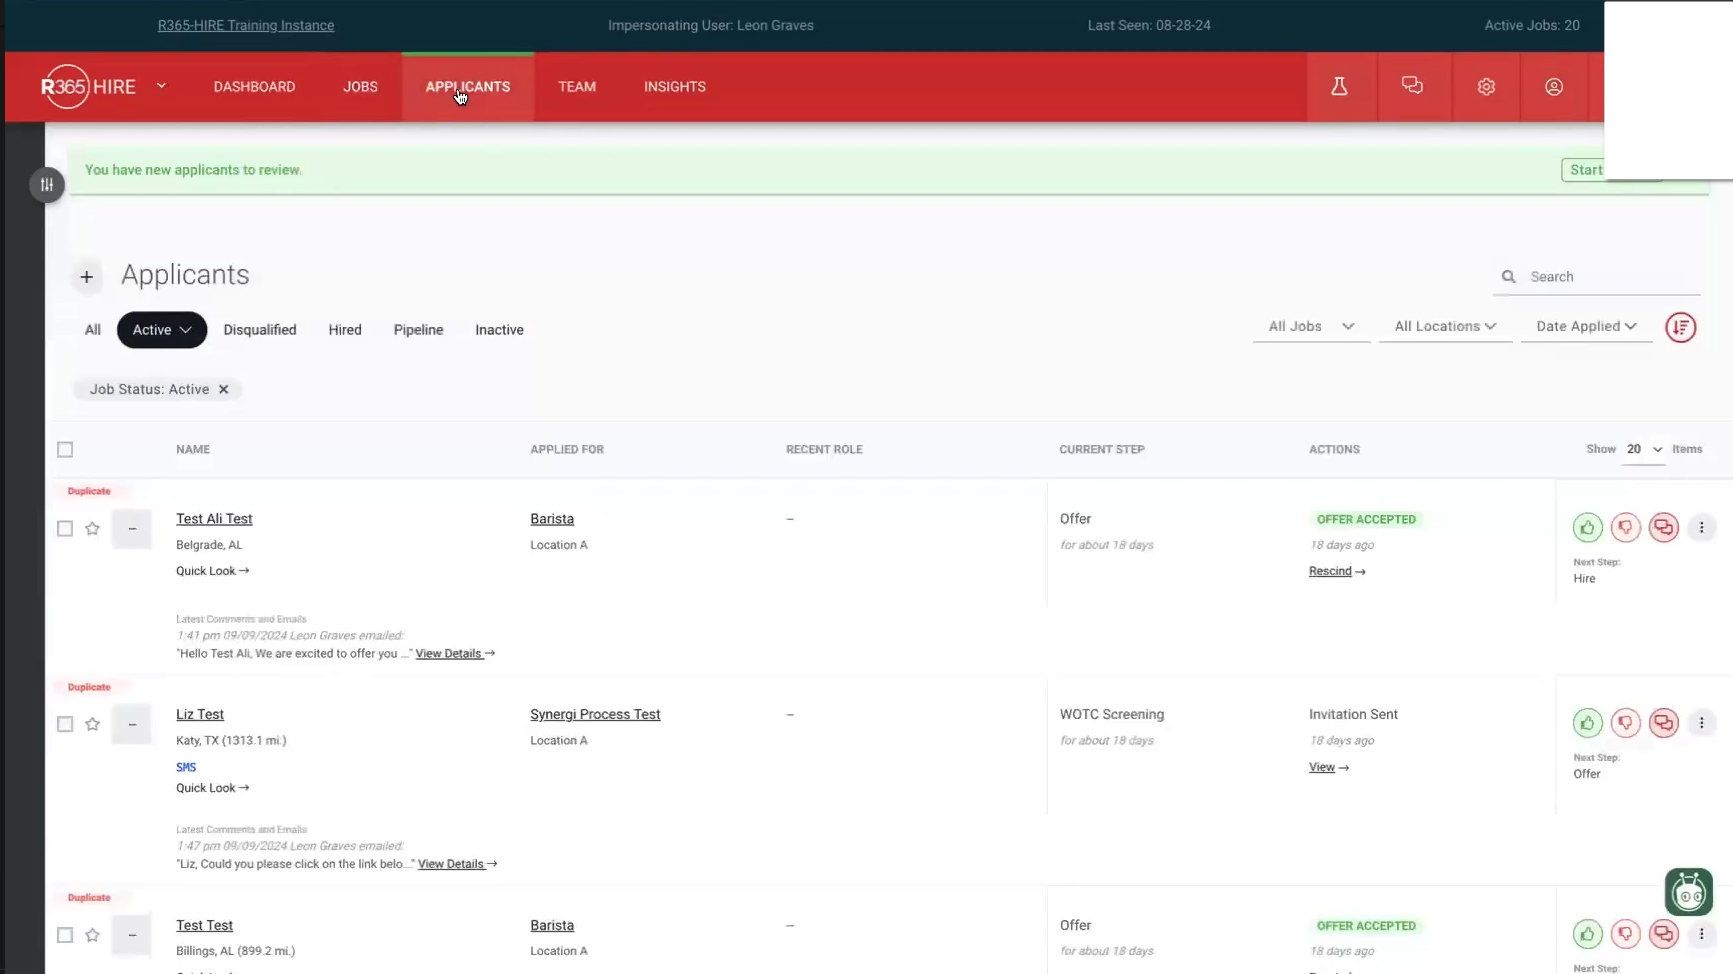
\includegraphics[width=\textwidth]{images/examples/applicants_r365.png}
        \caption{Applicants management interface (Restaurant365)}
    \end{minipage}
    \hfill
    \begin{minipage}{0.48\textwidth}
        \centering
        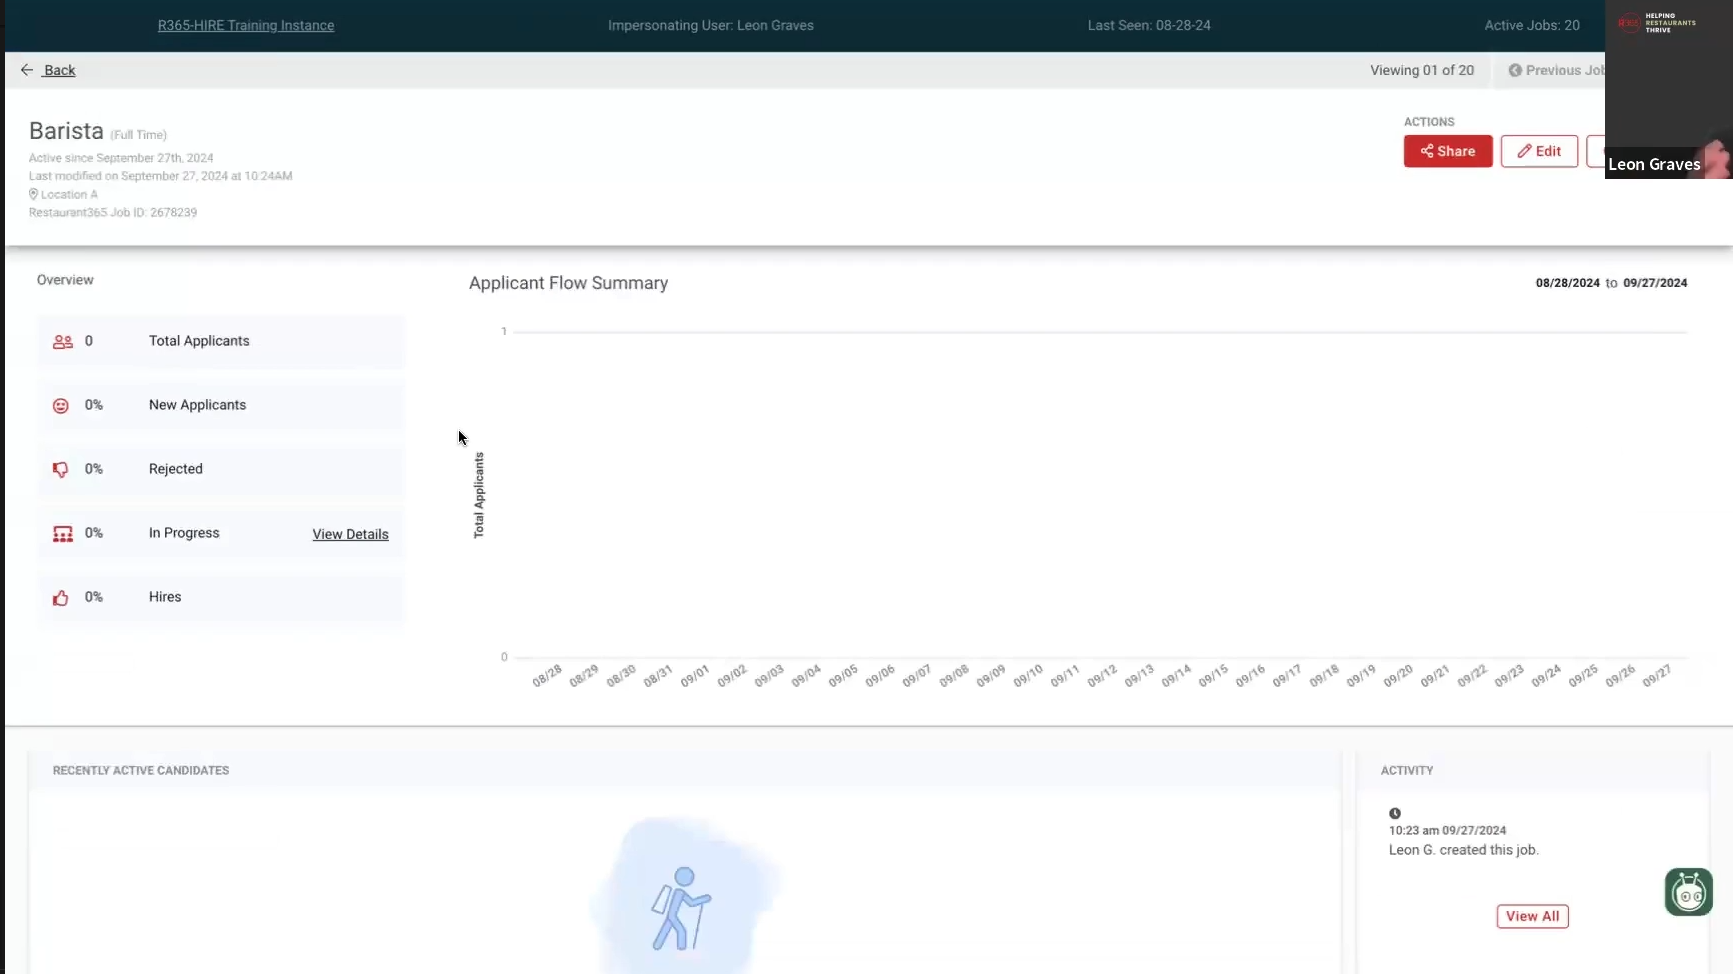
\includegraphics[width=\textwidth]{images/examples/hiring_status_r365.png}
        \caption{Hiring status overview (Restaurant365)}
    \end{minipage}
\end{figure}

\begin{figure}[h]
    \centering
    \begin{minipage}{0.48\textwidth}
        \centering
        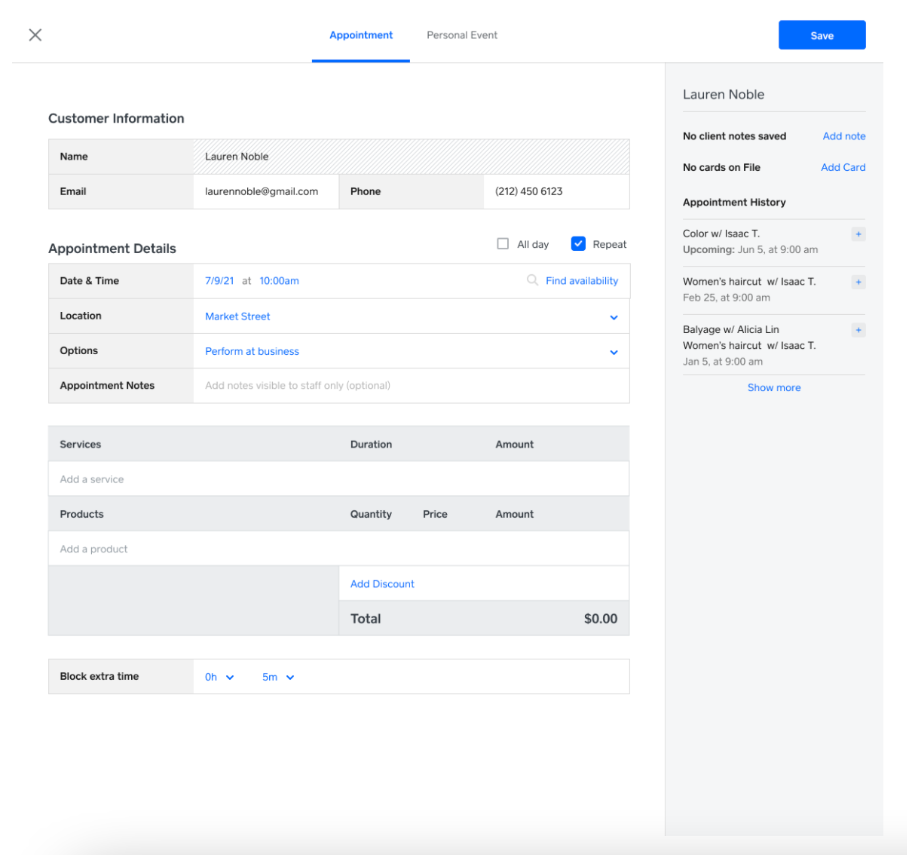
\includegraphics[width=\textwidth]{images/examples/appointment_creating_square.png}
        \caption{Appointment creation interface (Square)}
    \end{minipage}
    \hfill
    \begin{minipage}{0.48\textwidth}
        \centering
        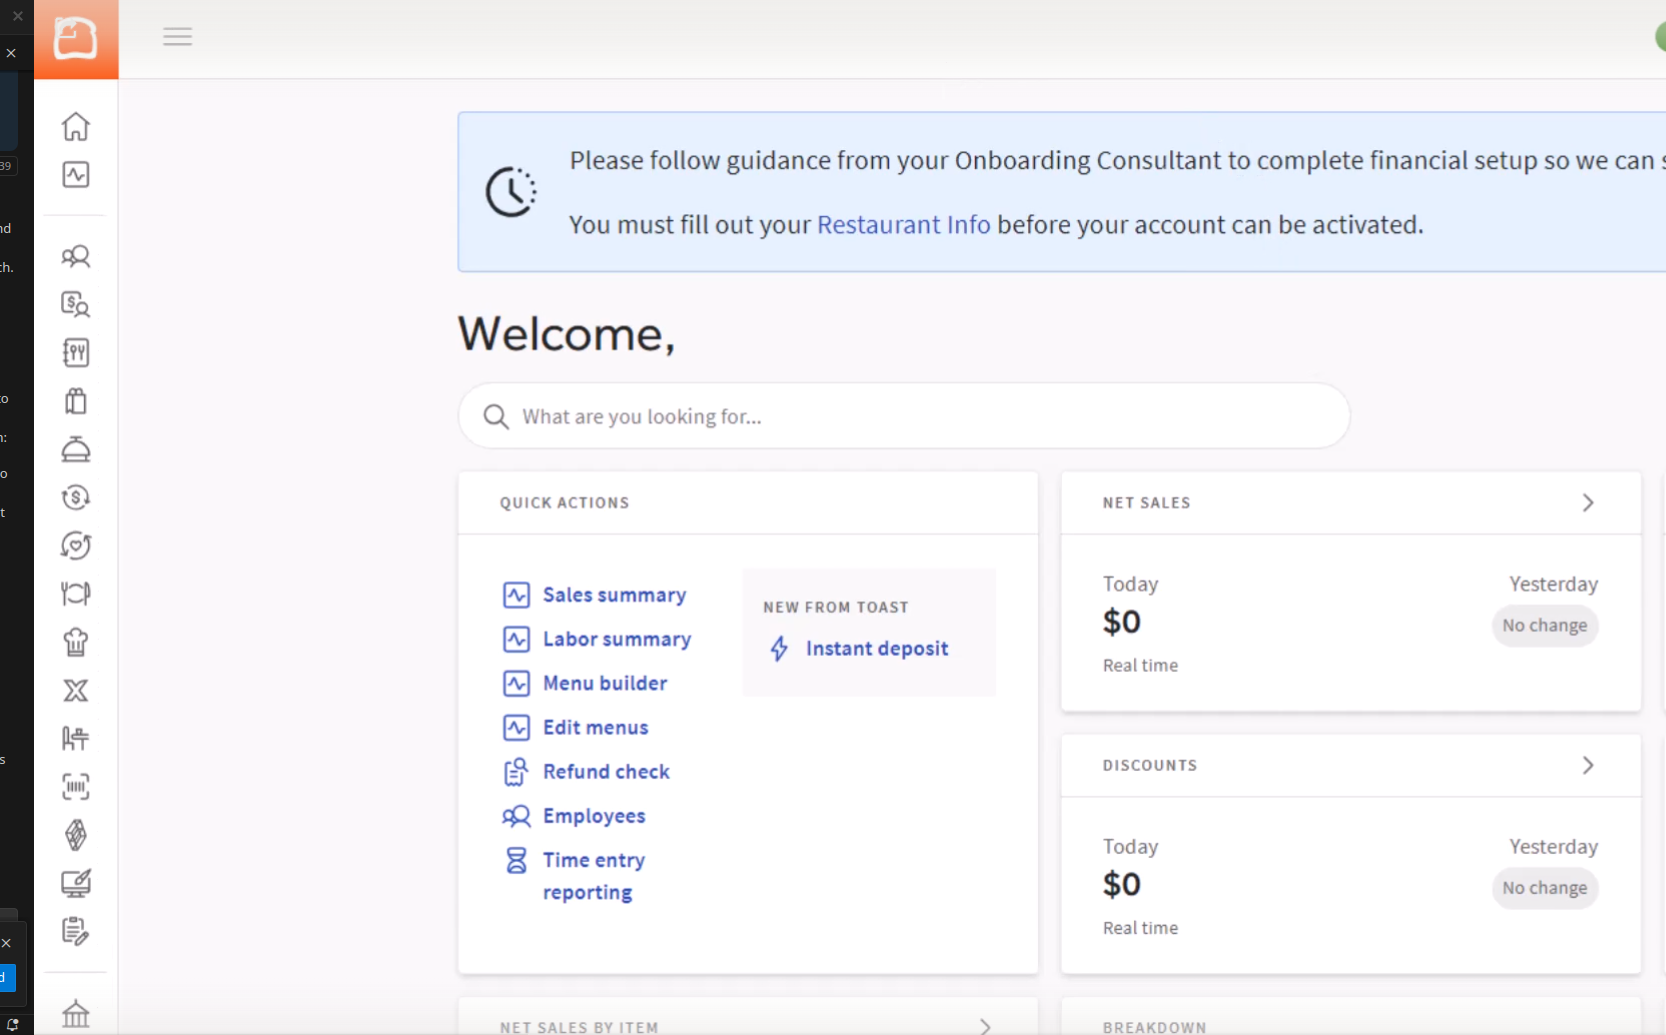
\includegraphics[width=\textwidth]{images/examples/homapage_toast.png}
        \caption{Homepage overview (Toast)}
    \end{minipage}
\end{figure}

\begin{figure}[h]
    \centering
    \begin{minipage}{0.48\textwidth}
        \centering
        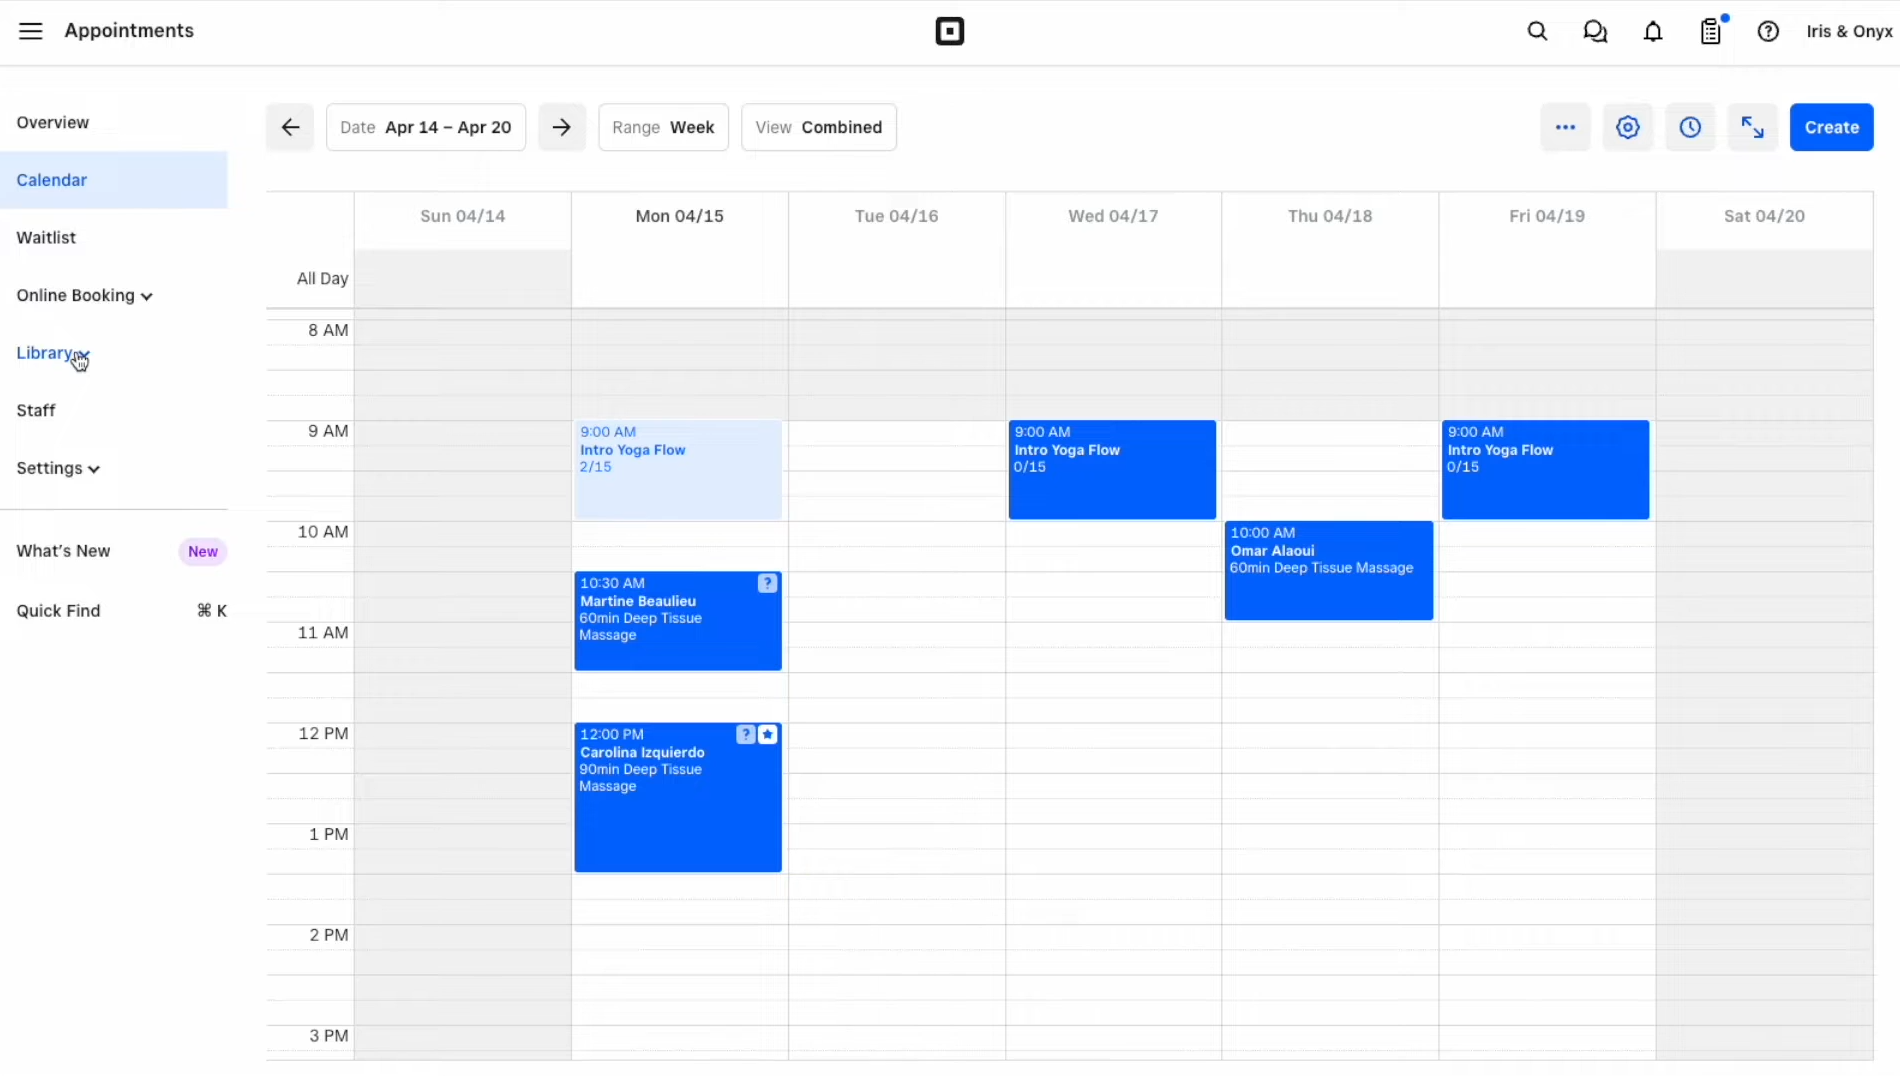
\includegraphics[width=\textwidth]{images/examples/appointments_square.png}
        \caption{Appointments list (Square)}
    \end{minipage}
    \hfill
    \begin{minipage}{0.48\textwidth}
        \centering
        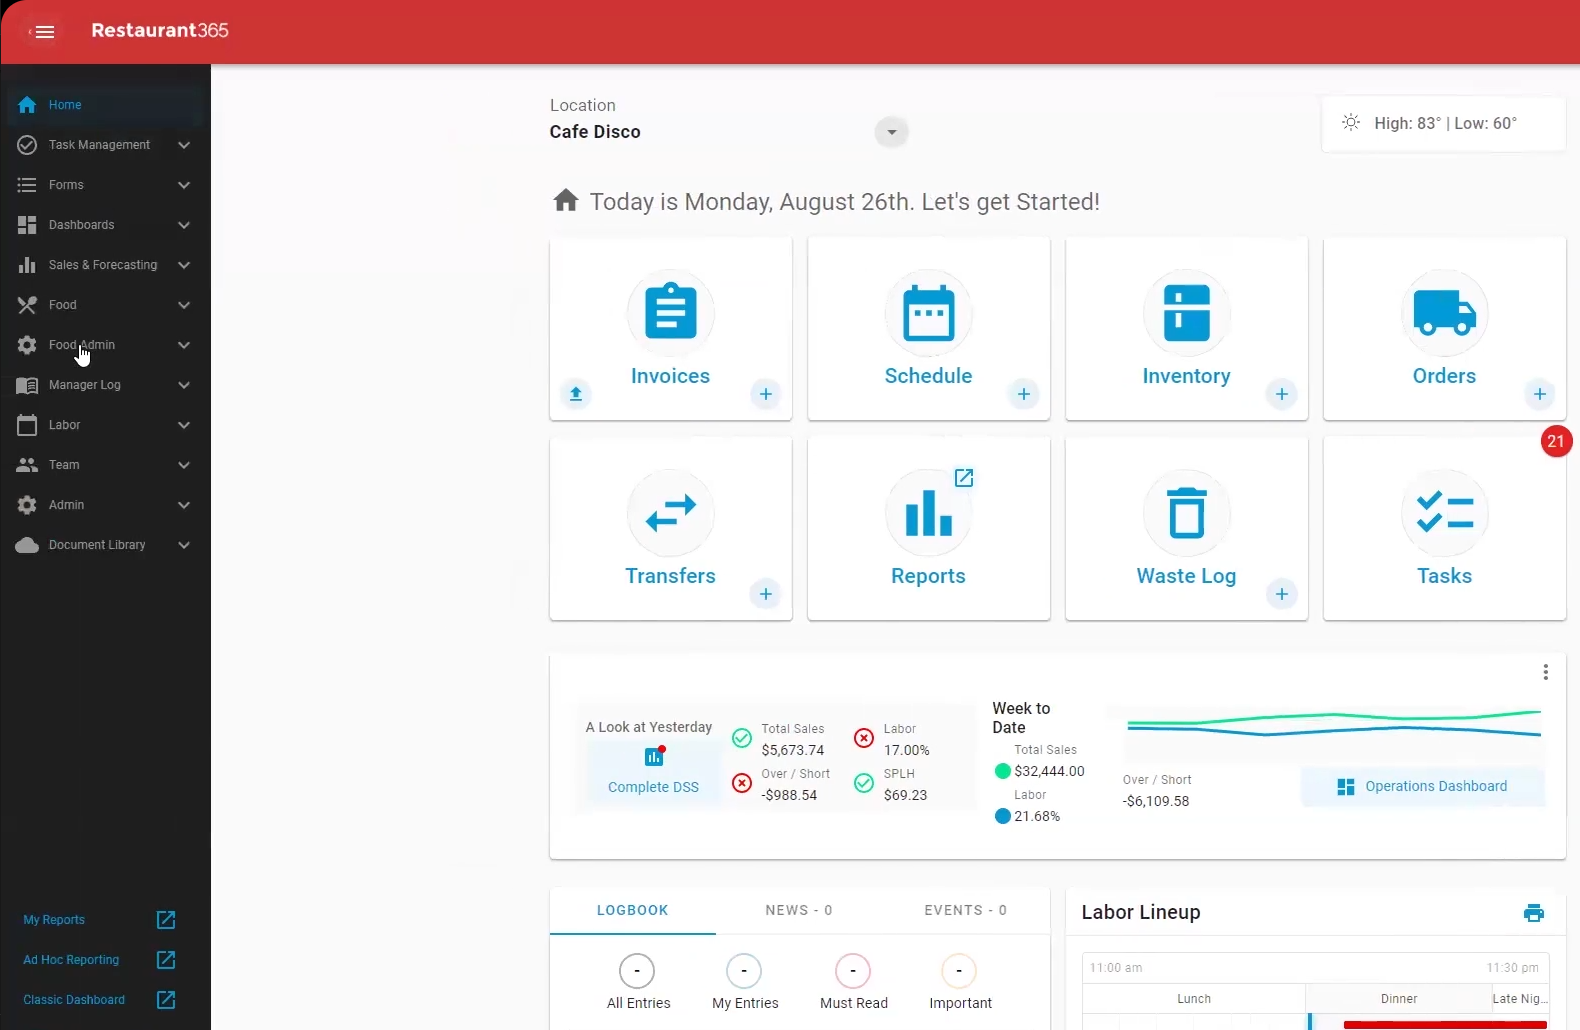
\includegraphics[width=\textwidth]{images/examples/homepage_r365.png}
        \caption{Homepage dashboard (Restaurant365)}
    \end{minipage}
\end{figure}

\begin{figure}[h]
    \centering
    \begin{minipage}{0.48\textwidth}
        \centering
        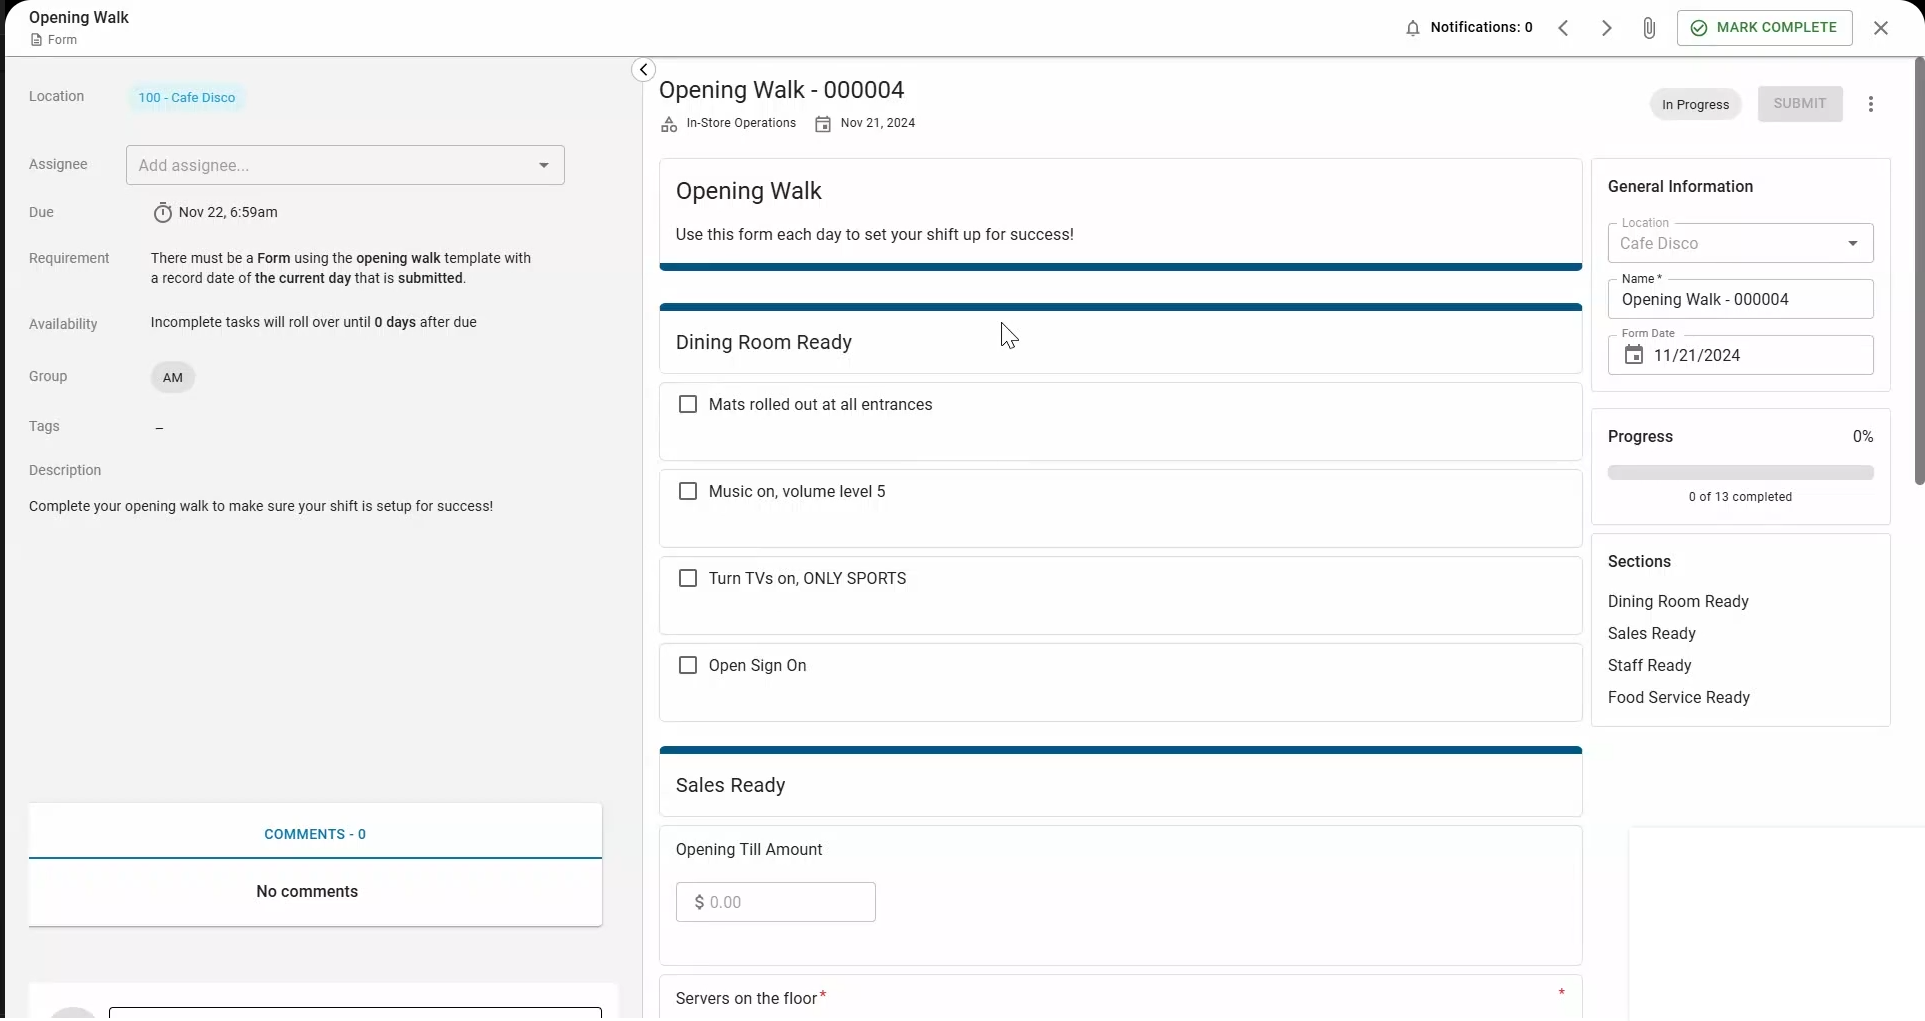
\includegraphics[width=\textwidth]{images/examples/forms_r365.png}
        \caption{Forms management (Restaurant365)}
    \end{minipage}
    \hfill
    \begin{minipage}{0.48\textwidth}
        \centering
        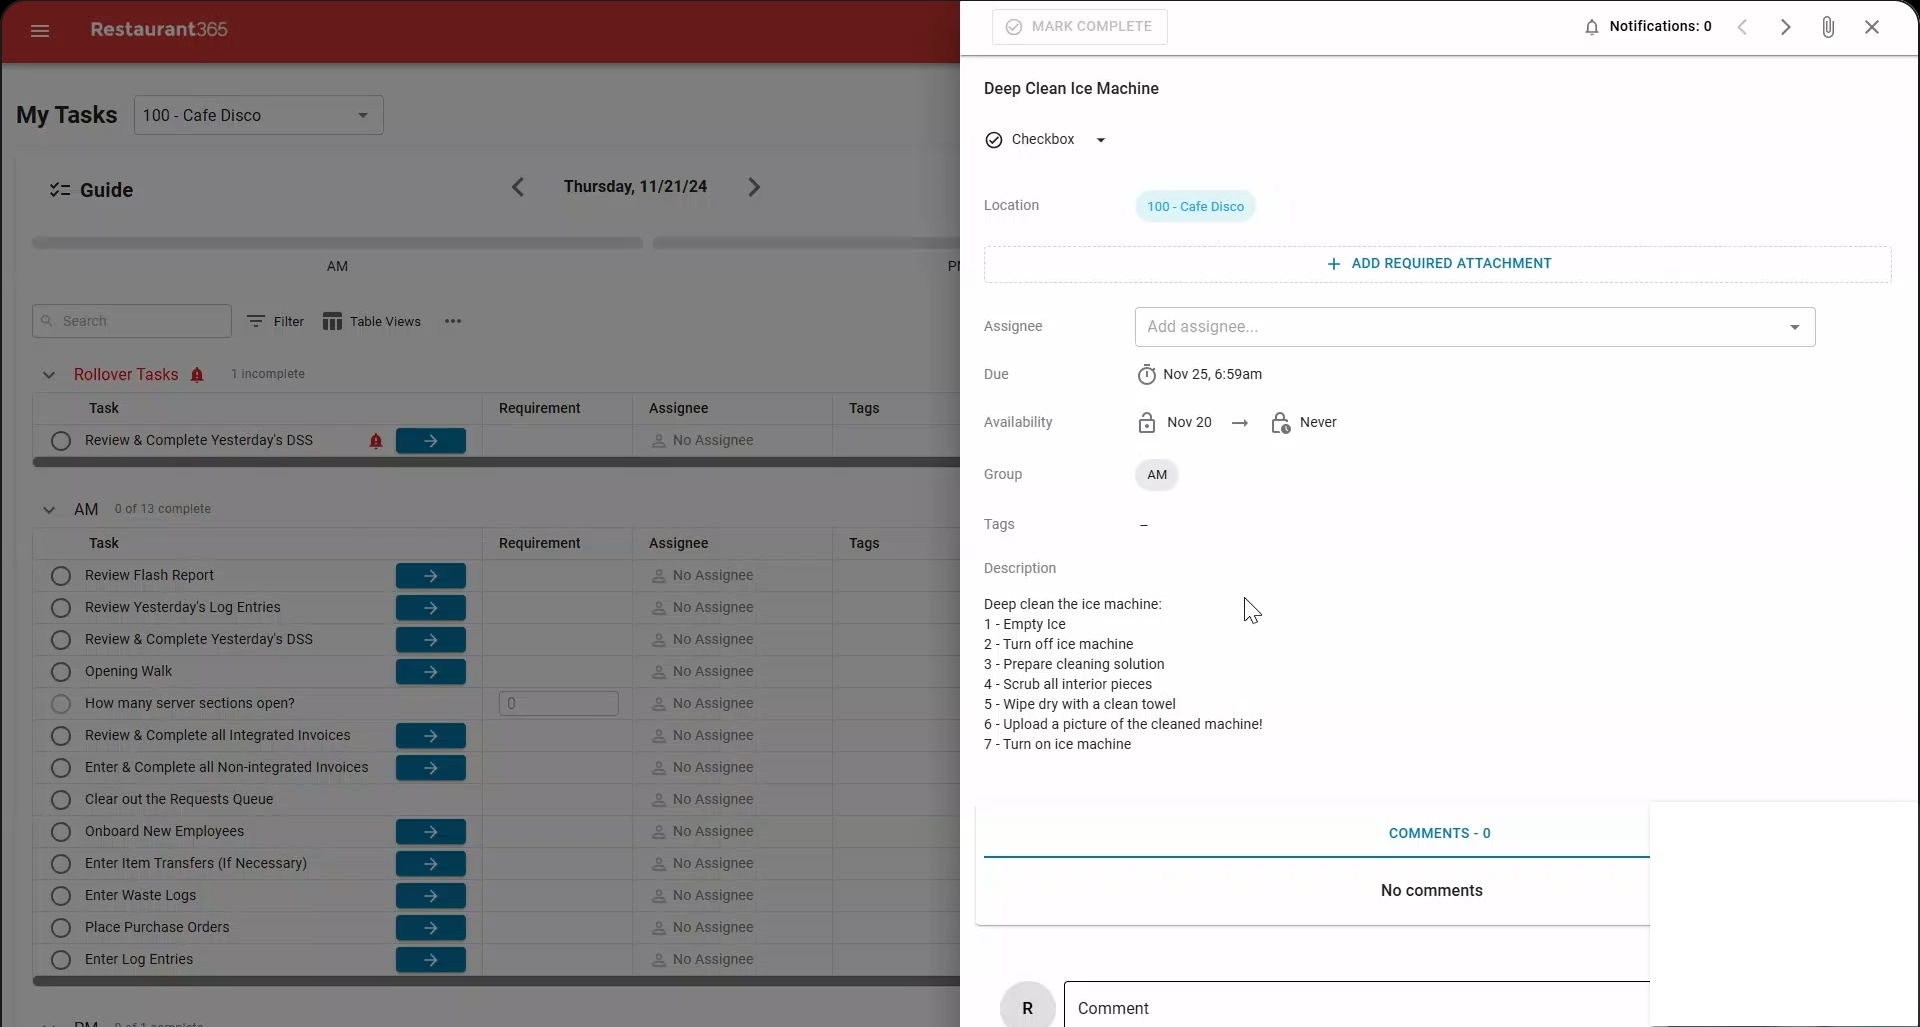
\includegraphics[width=\textwidth]{images/examples/image.png}
        \caption{General interface example}
    \end{minipage}
\end{figure}

\begin{figure}[h]
    \centering
    \begin{minipage}{0.48\textwidth}
        \centering
        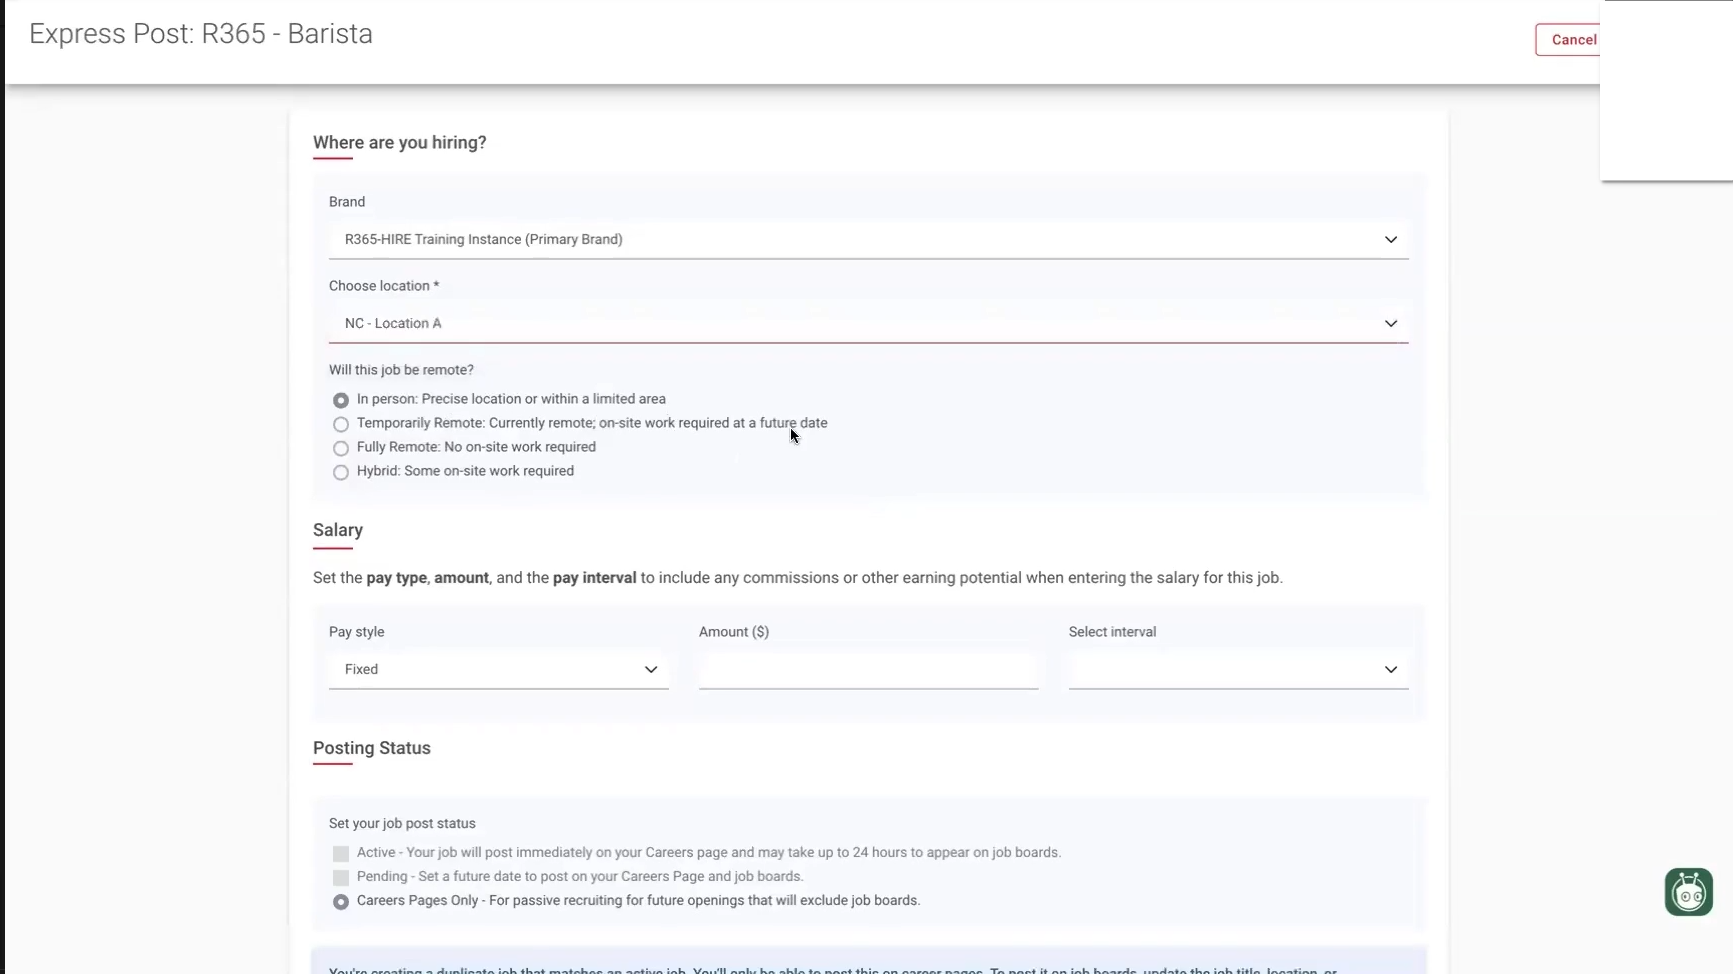
\includegraphics[width=\textwidth]{images/examples/hiring_r365.png}
        \caption{Hiring process overview (Restaurant365)}
    \end{minipage}
    \hfill
    \begin{minipage}{0.48\textwidth}
        \centering
        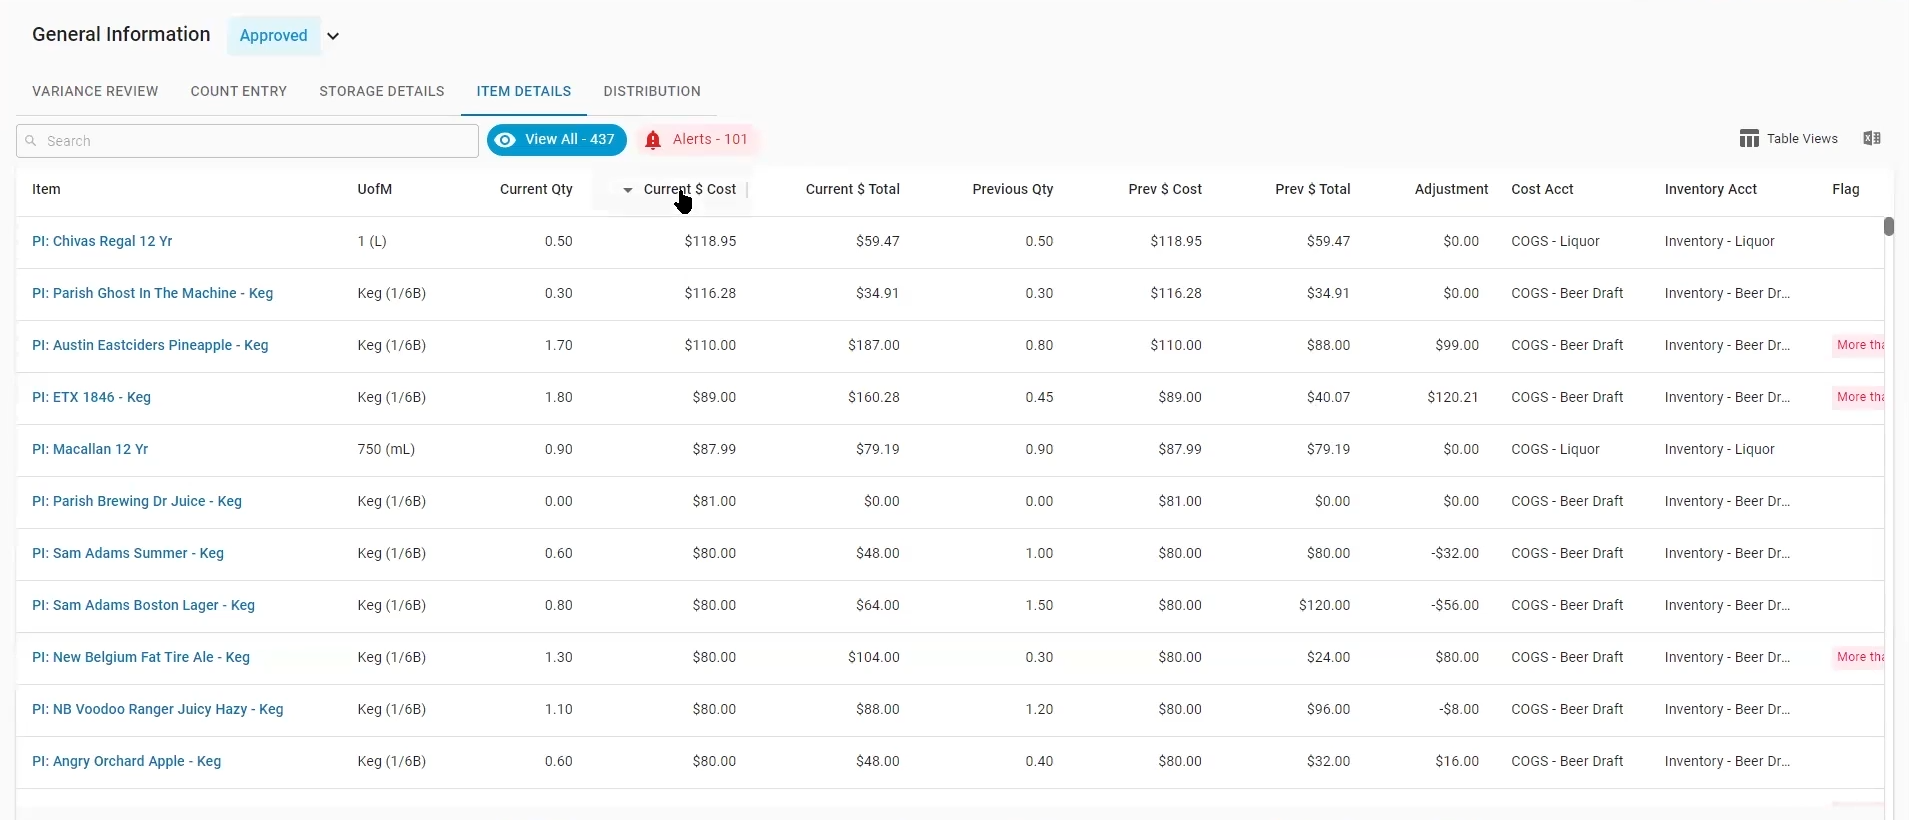
\includegraphics[width=\textwidth]{images/examples/inventory_r365.png}
        \caption{Inventory management (Restaurant365)}
    \end{minipage}
\end{figure}

\begin{figure}[h]
    \centering
    \begin{minipage}{0.48\textwidth}
        \centering
        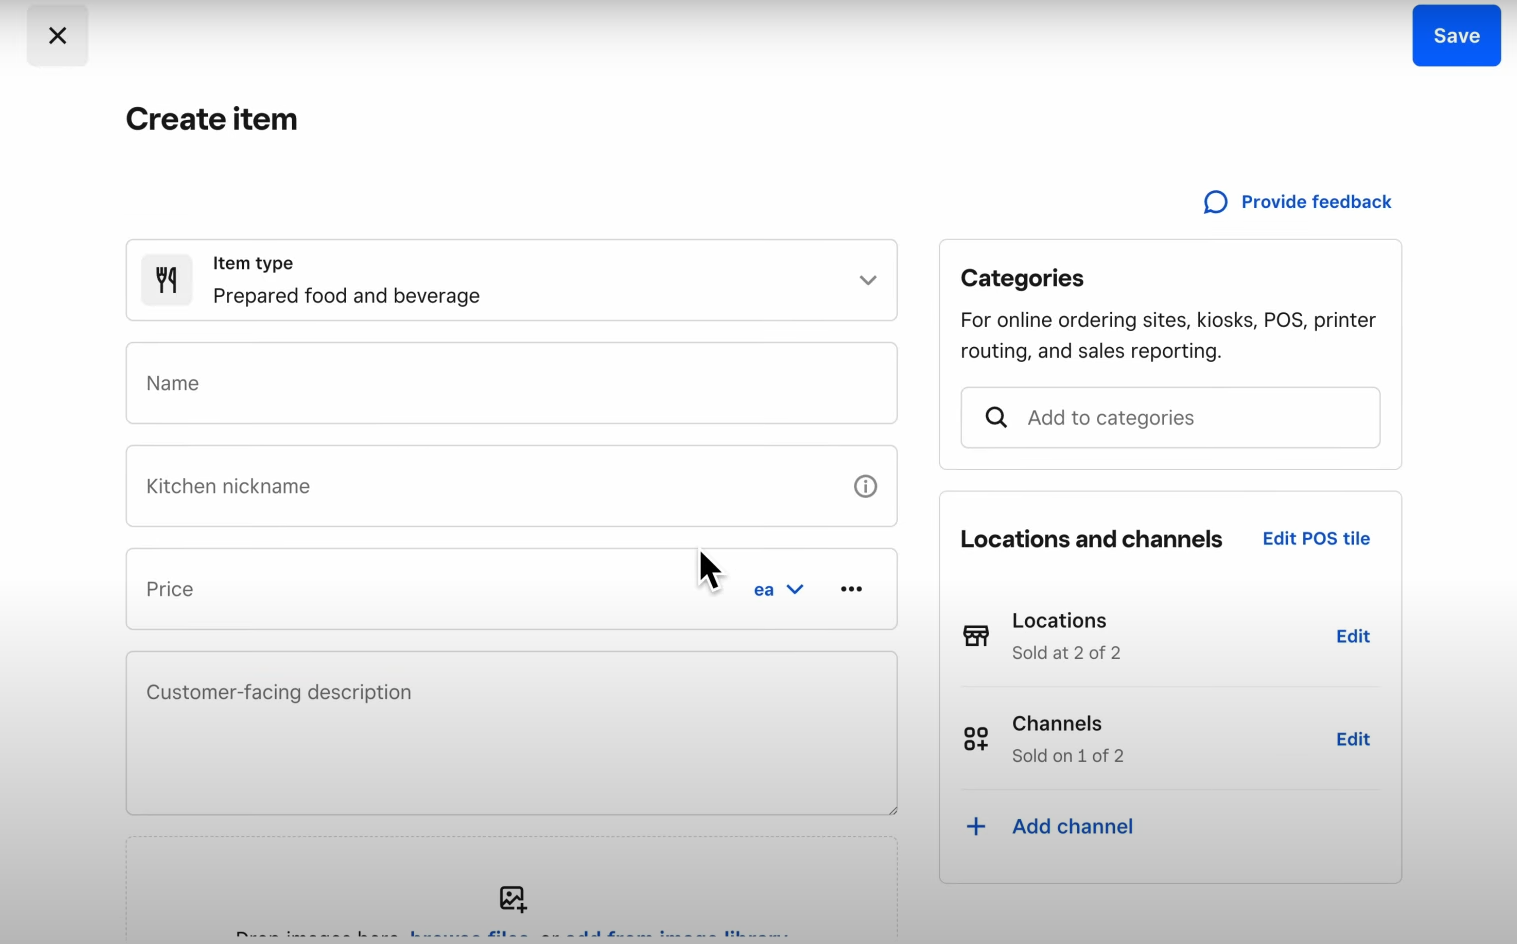
\includegraphics[width=\textwidth]{images/examples/item_creating_square.png}
        \caption{Item creation interface (Square)}
    \end{minipage}
    \hfill
    \begin{minipage}{0.48\textwidth}
        \centering
        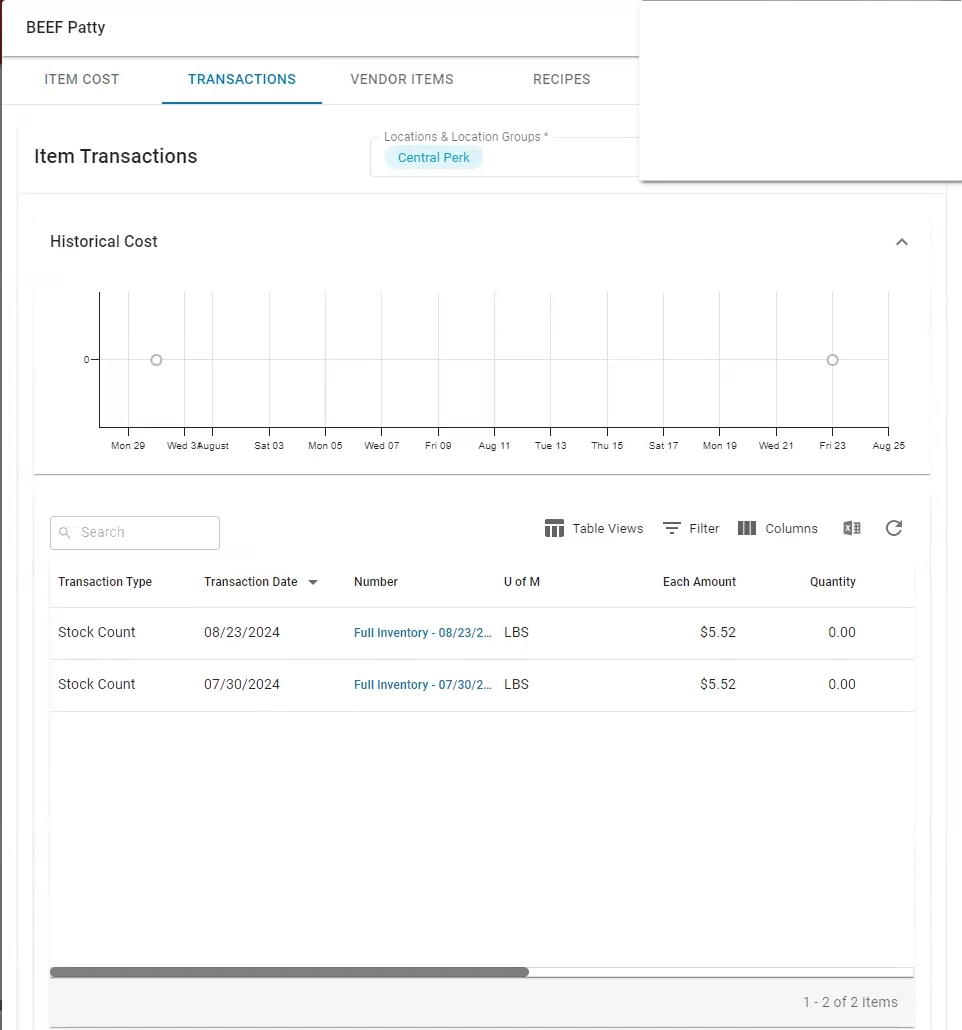
\includegraphics[width=\textwidth]{images/examples/item_transactions_r365.png}
        \caption{Item transactions (Restaurant365)}
    \end{minipage}
\end{figure}

\begin{figure}[h]
    \centering
    \begin{minipage}{0.48\textwidth}
        \centering
        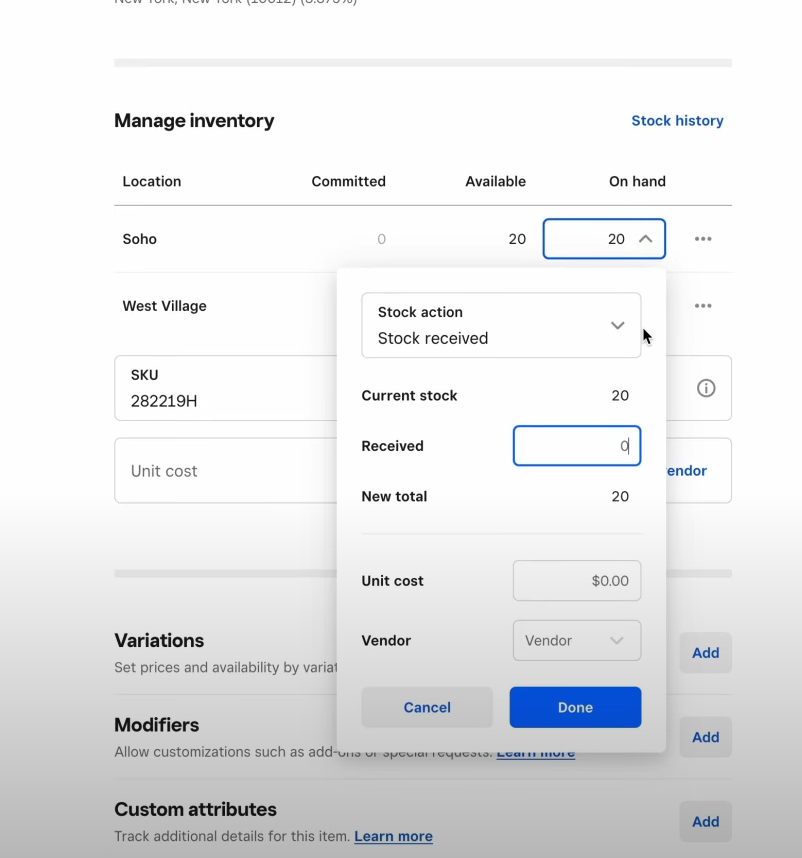
\includegraphics[width=\textwidth]{images/examples/item_inventory_square.png}
        \caption{Item inventory view (Square)}
    \end{minipage}
    \hfill
    \begin{minipage}{0.48\textwidth}
        \centering
        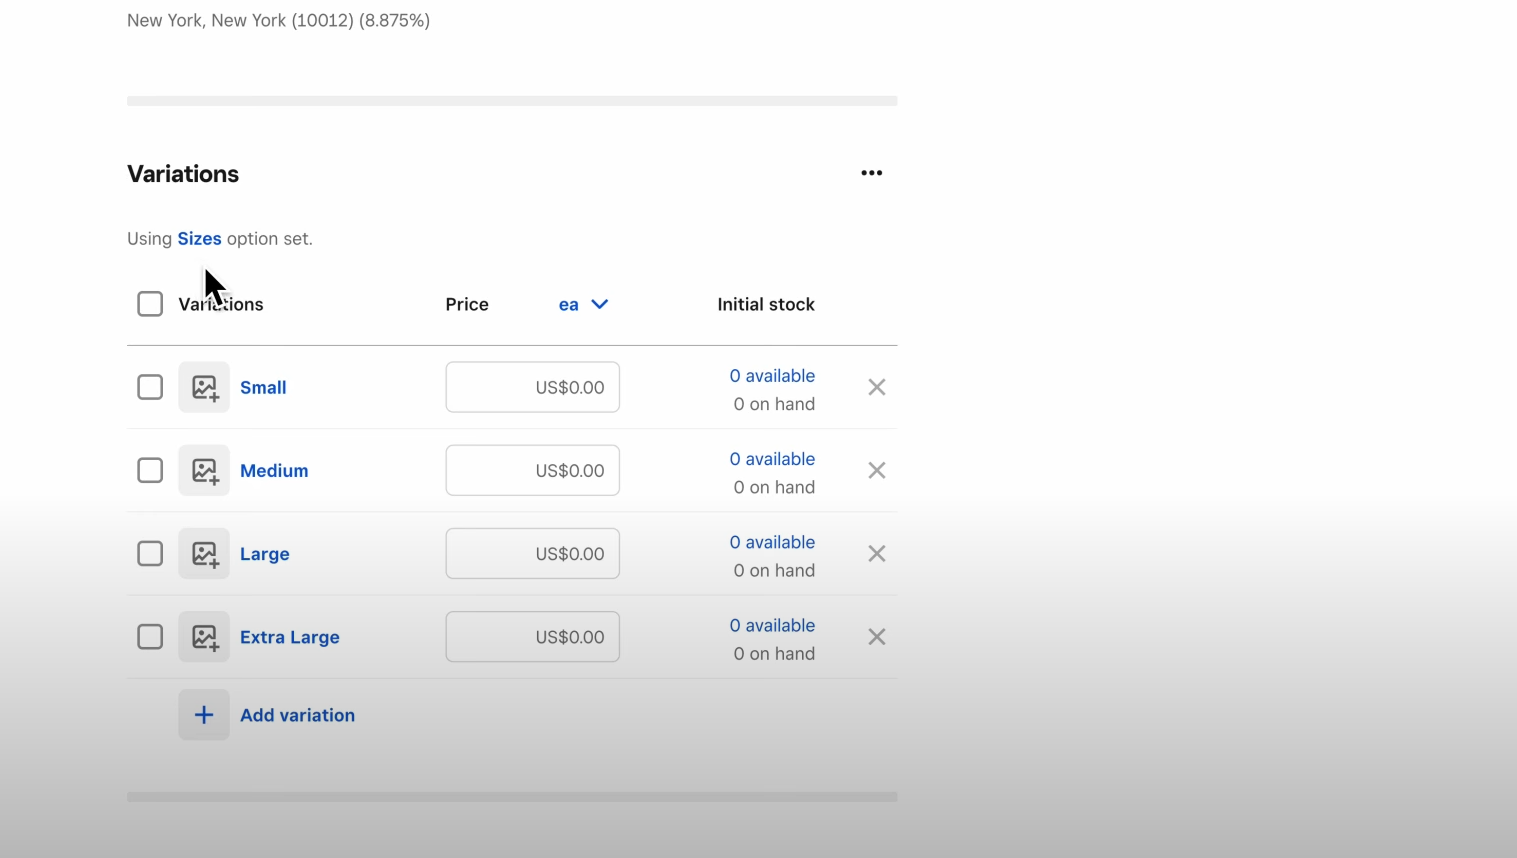
\includegraphics[width=\textwidth]{images/examples/item_variations_square.png}
        \caption{Item variations (Square)}
    \end{minipage}
\end{figure}

\begin{figure}[h]
    \centering
    \begin{minipage}{0.48\textwidth}
        \centering
        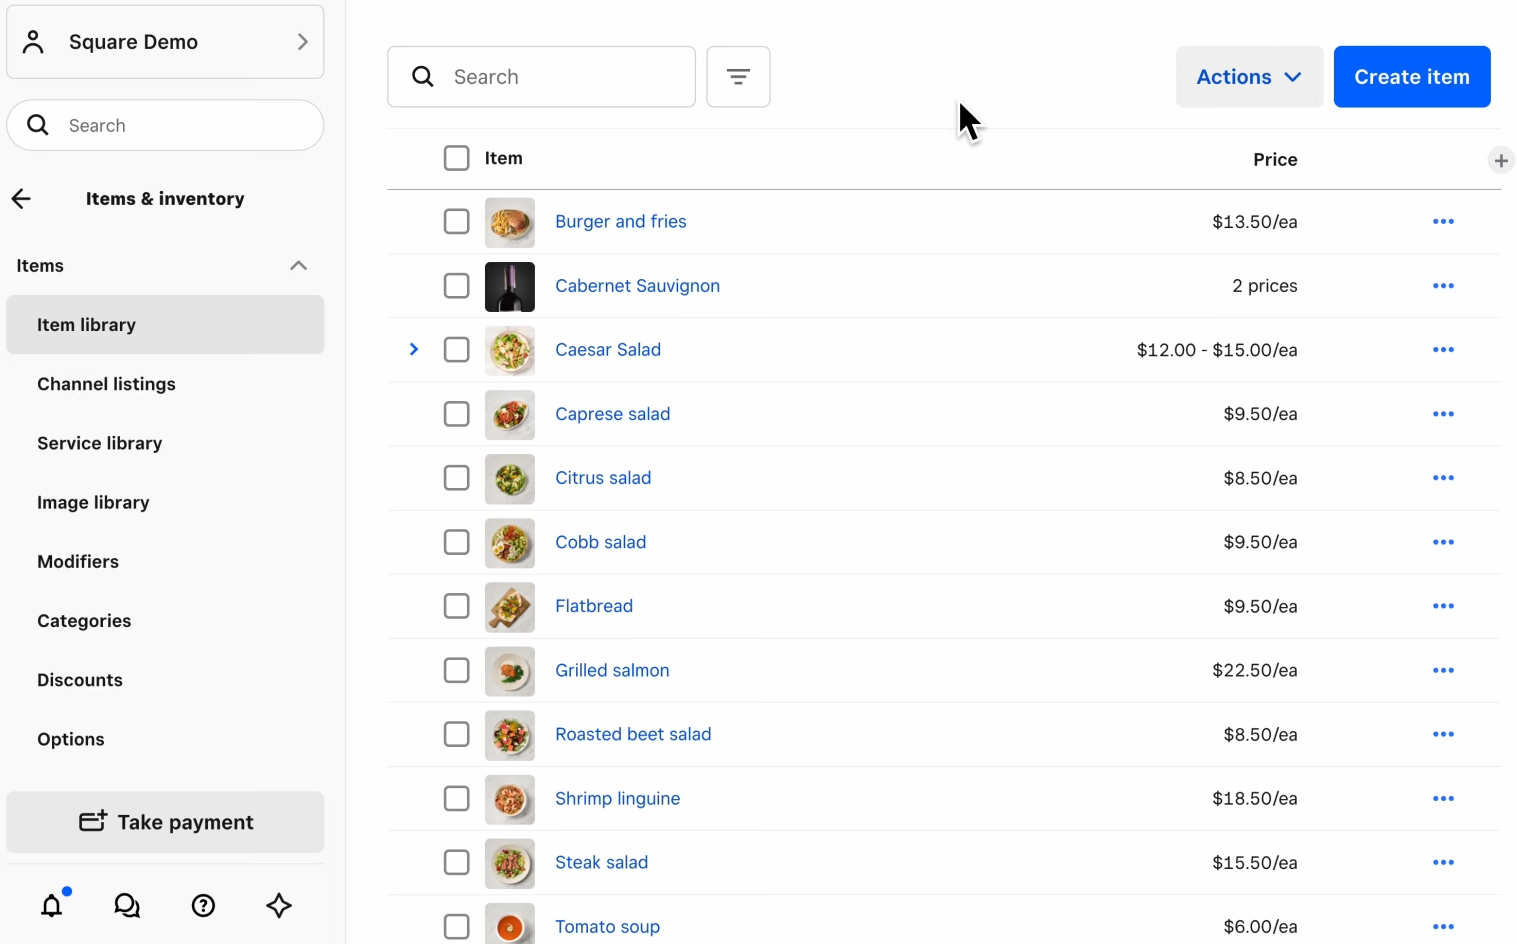
\includegraphics[width=\textwidth]{images/examples/item_menu_square.png}
        \caption{Menu item configuration (Square)}
    \end{minipage}
    \hfill
    \begin{minipage}{0.48\textwidth}
        \centering
        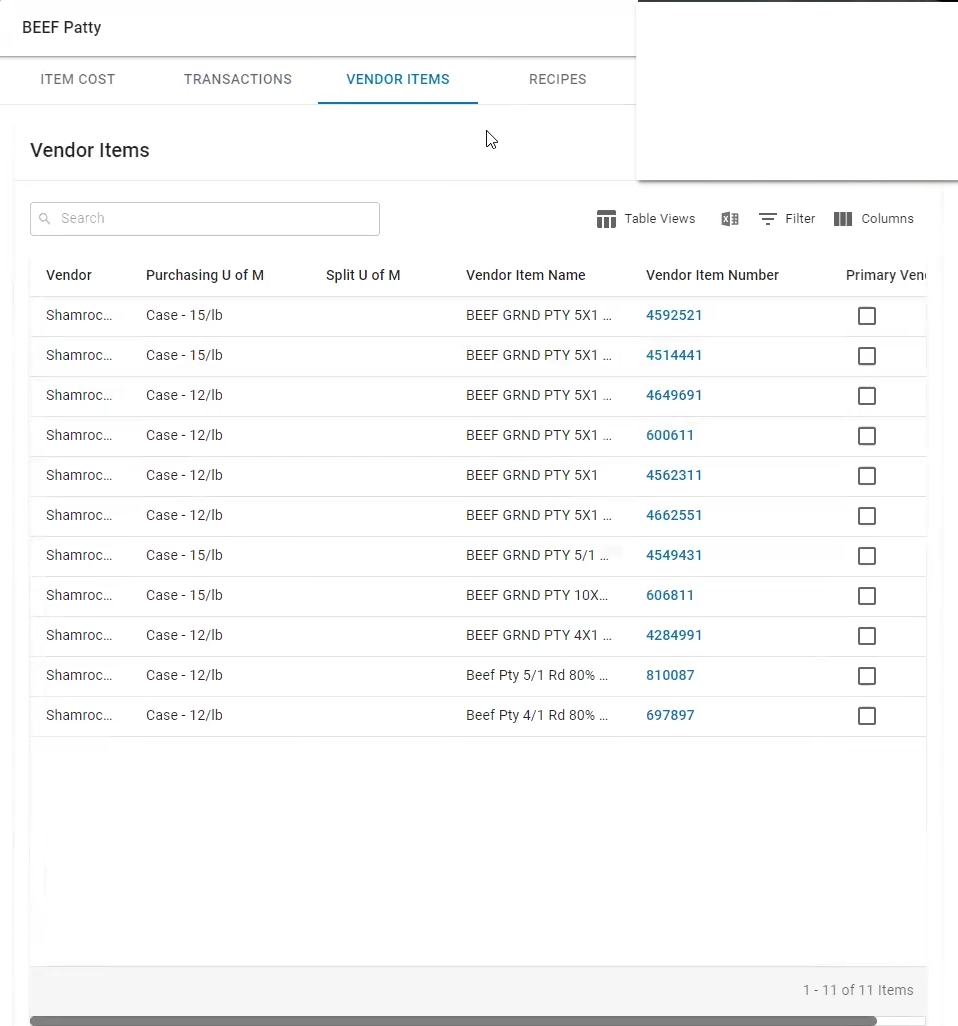
\includegraphics[width=\textwidth]{images/examples/item_vendor_items_r365.png}
        \caption{Vendor items management (Restaurant365)}
    \end{minipage}
\end{figure}

\begin{figure}[h]
    \centering
    \begin{minipage}{0.48\textwidth}
        \centering
        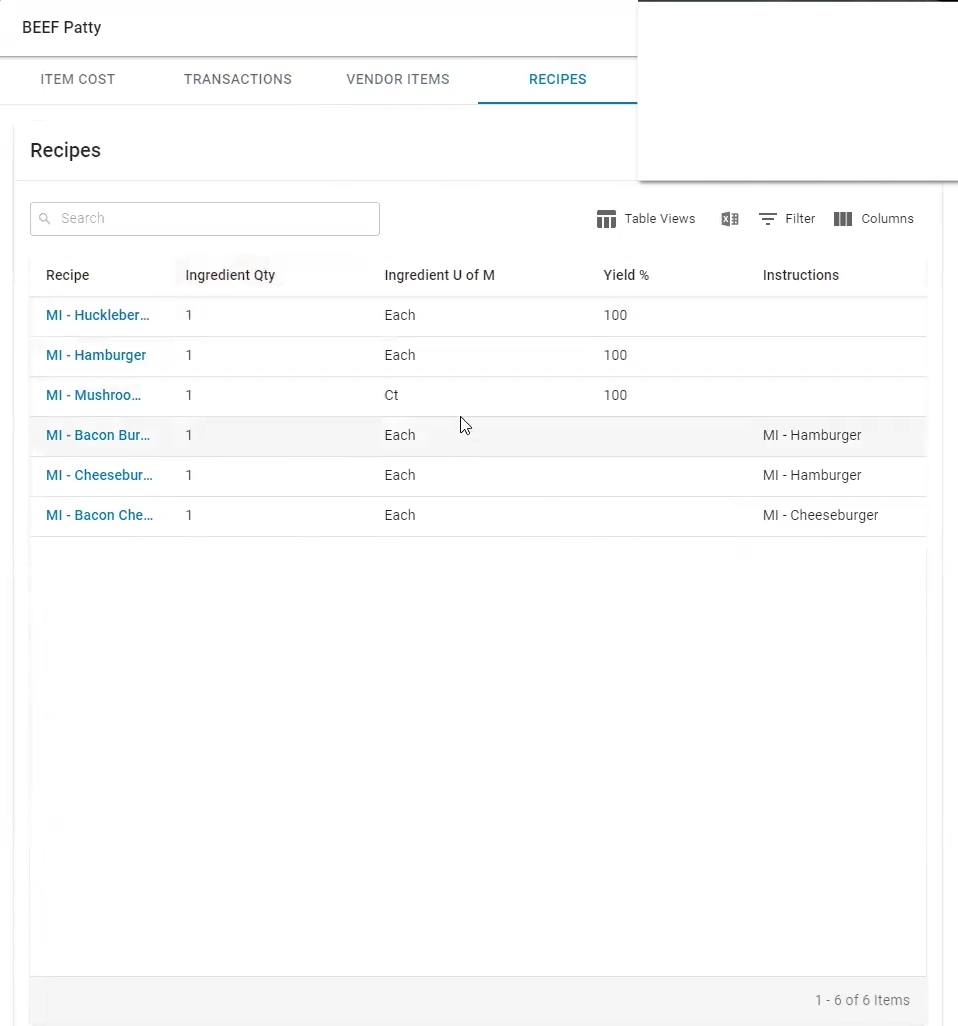
\includegraphics[width=\textwidth]{images/examples/item_recipes_r365.png}
        \caption{Recipe management (Restaurant365)}
    \end{minipage}
    \hfill
    \begin{minipage}{0.48\textwidth}
        \centering
        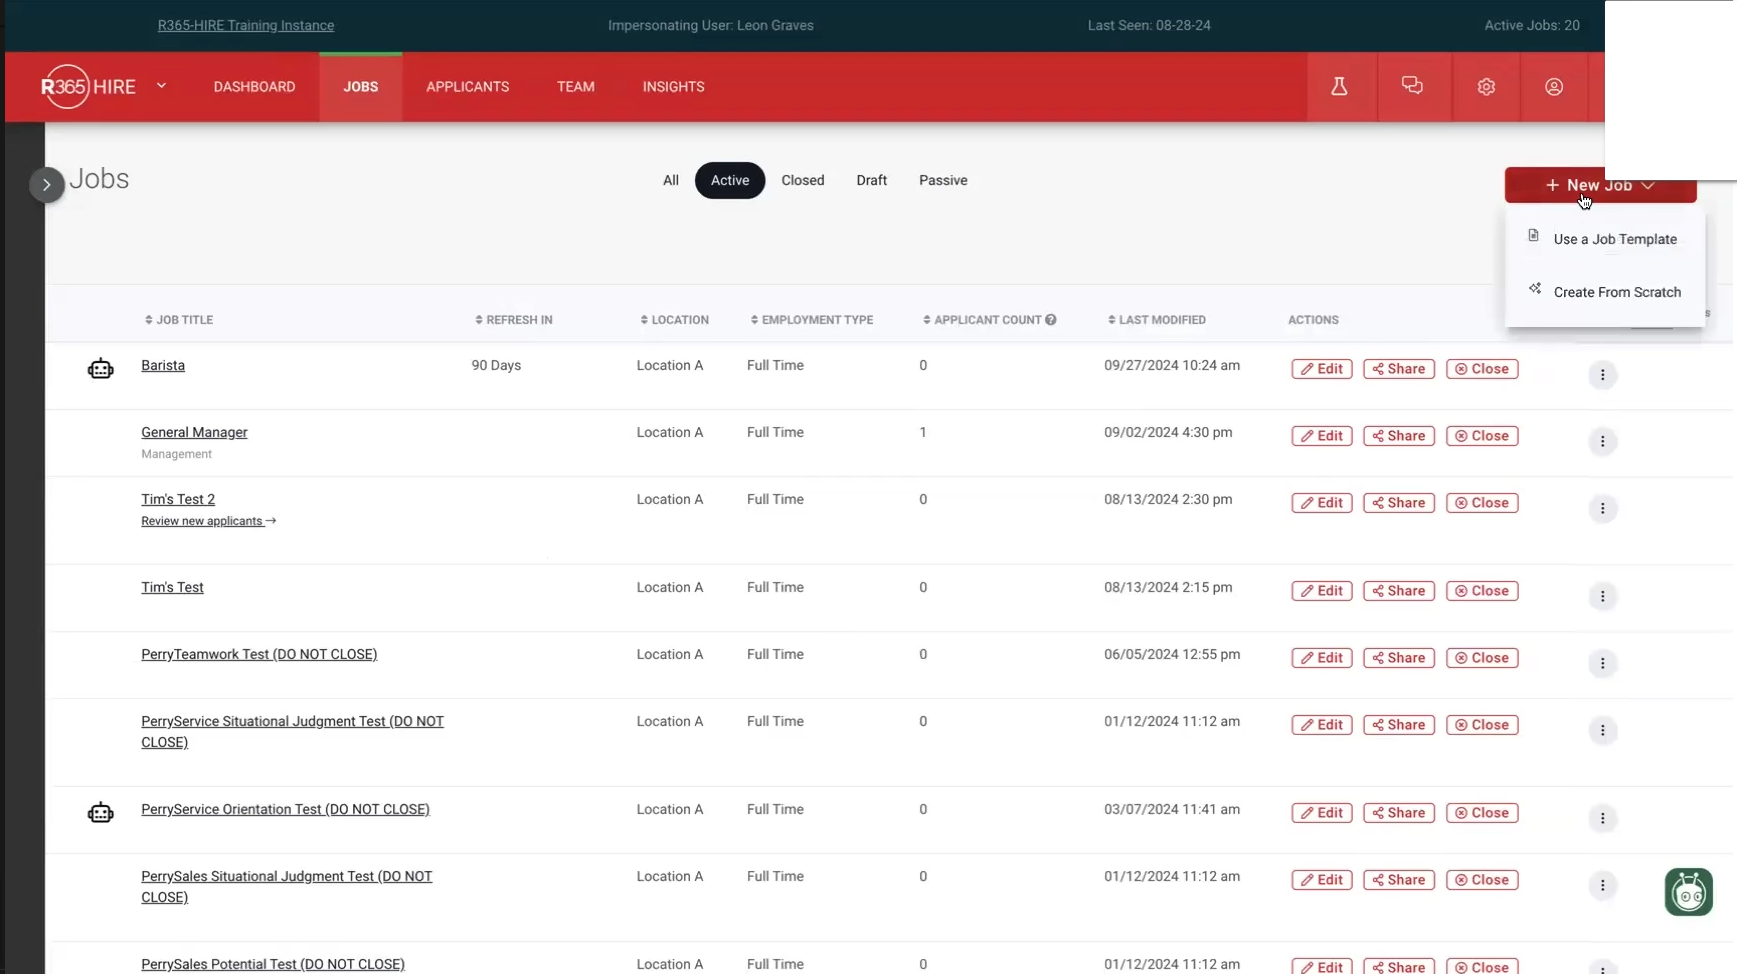
\includegraphics[width=\textwidth]{images/examples/jobs_r365.png}
        \caption{Jobs overview (Restaurant365)}
    \end{minipage}
\end{figure}

\begin{figure}[h]
    \centering
    \begin{minipage}{0.48\textwidth}
        \centering
        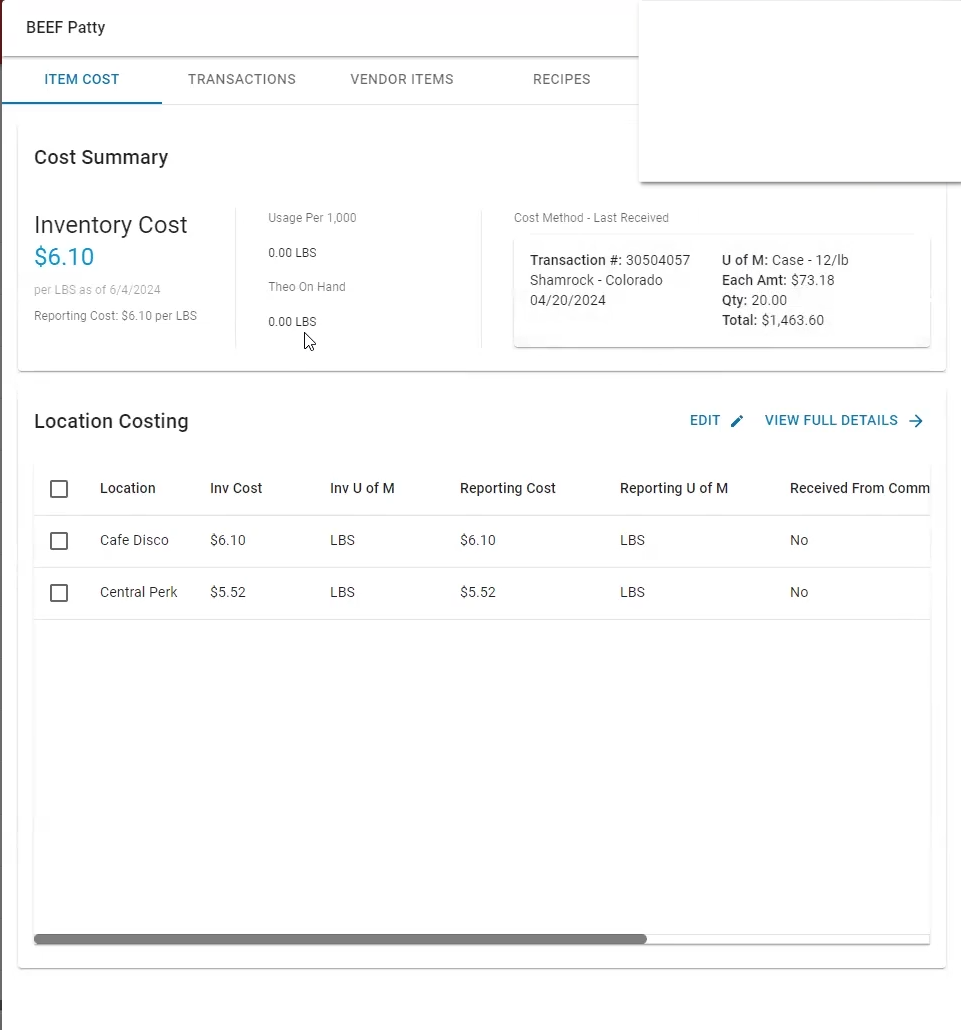
\includegraphics[width=\textwidth]{images/examples/items_cost_r365.png}
        \caption{Items cost analysis (Restaurant365)}
    \end{minipage}
    \hfill
    \begin{minipage}{0.48\textwidth}
        \centering
        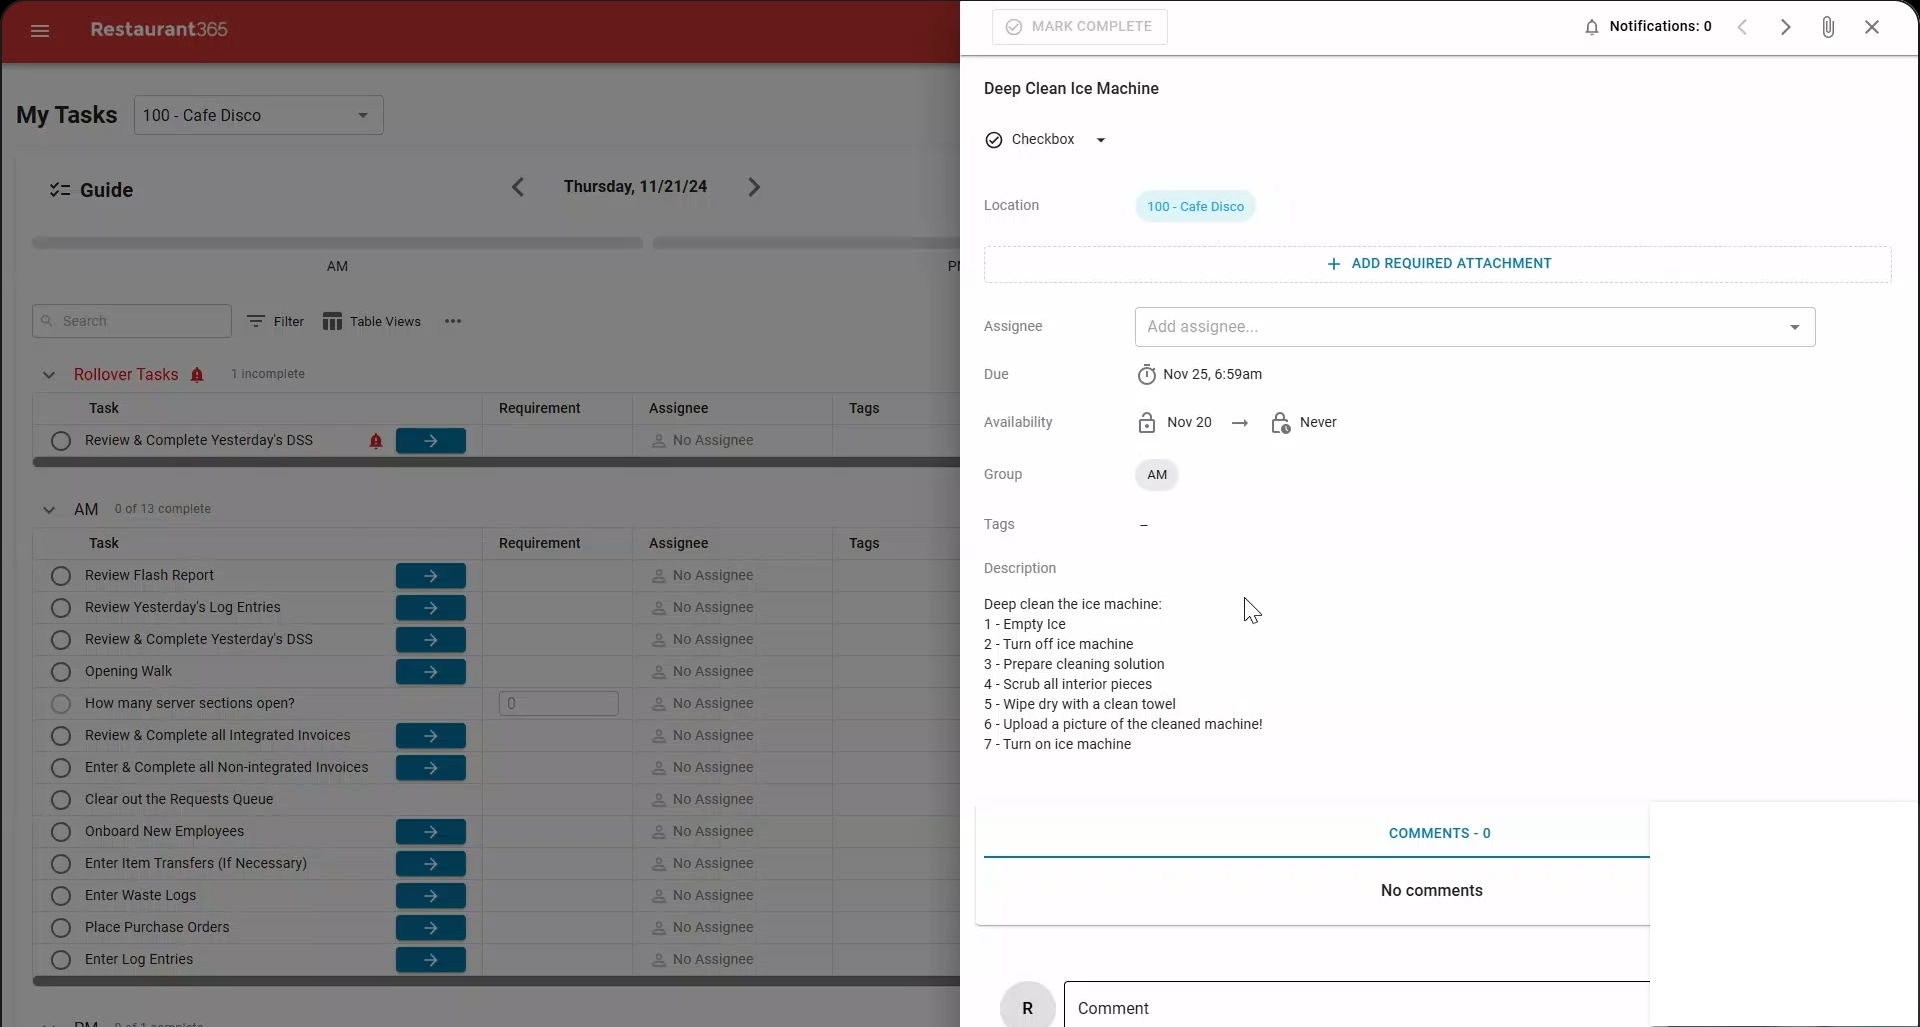
\includegraphics[width=\textwidth]{images/examples/more_tasks_r365.png}
        \caption{Task list (Restaurant365)}
    \end{minipage}
\end{figure}

\begin{figure}[h]
    \centering
    \begin{minipage}{0.48\textwidth}
        \centering
        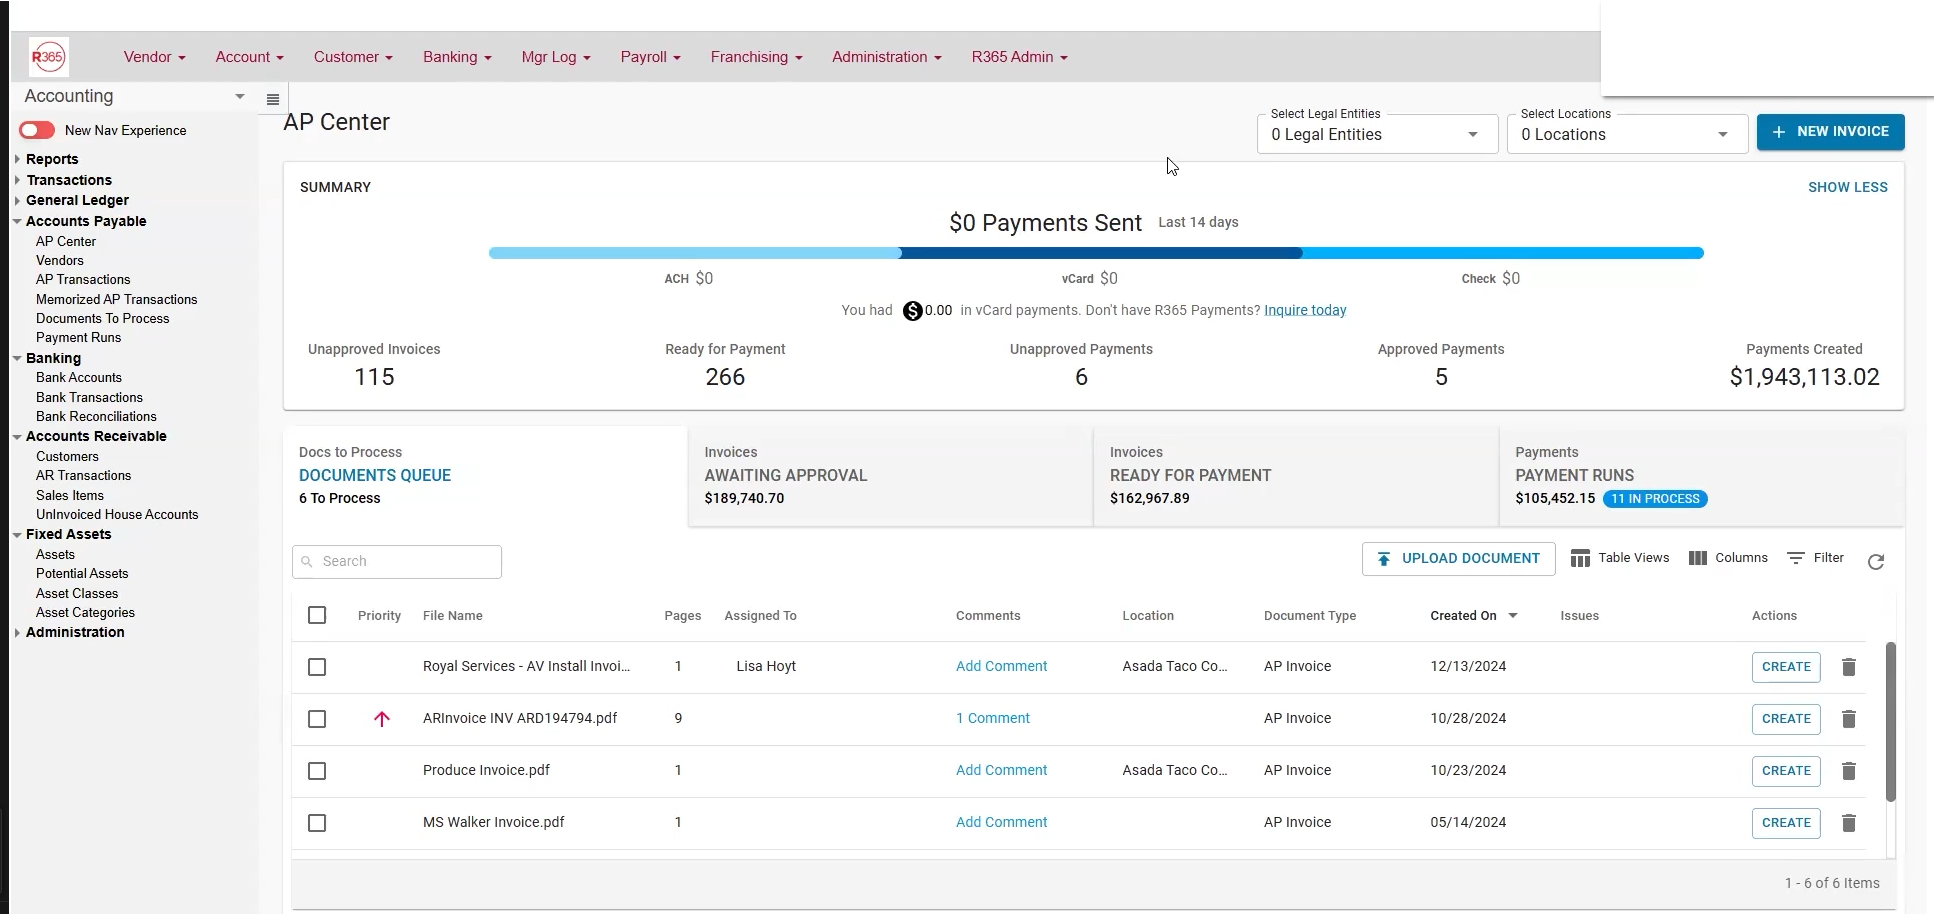
\includegraphics[width=\textwidth]{images/examples/payment_center_r365.png}
        \caption{Payment center (Restaurant365)}
    \end{minipage}
    \hfill
    \begin{minipage}{0.48\textwidth}
        \centering
        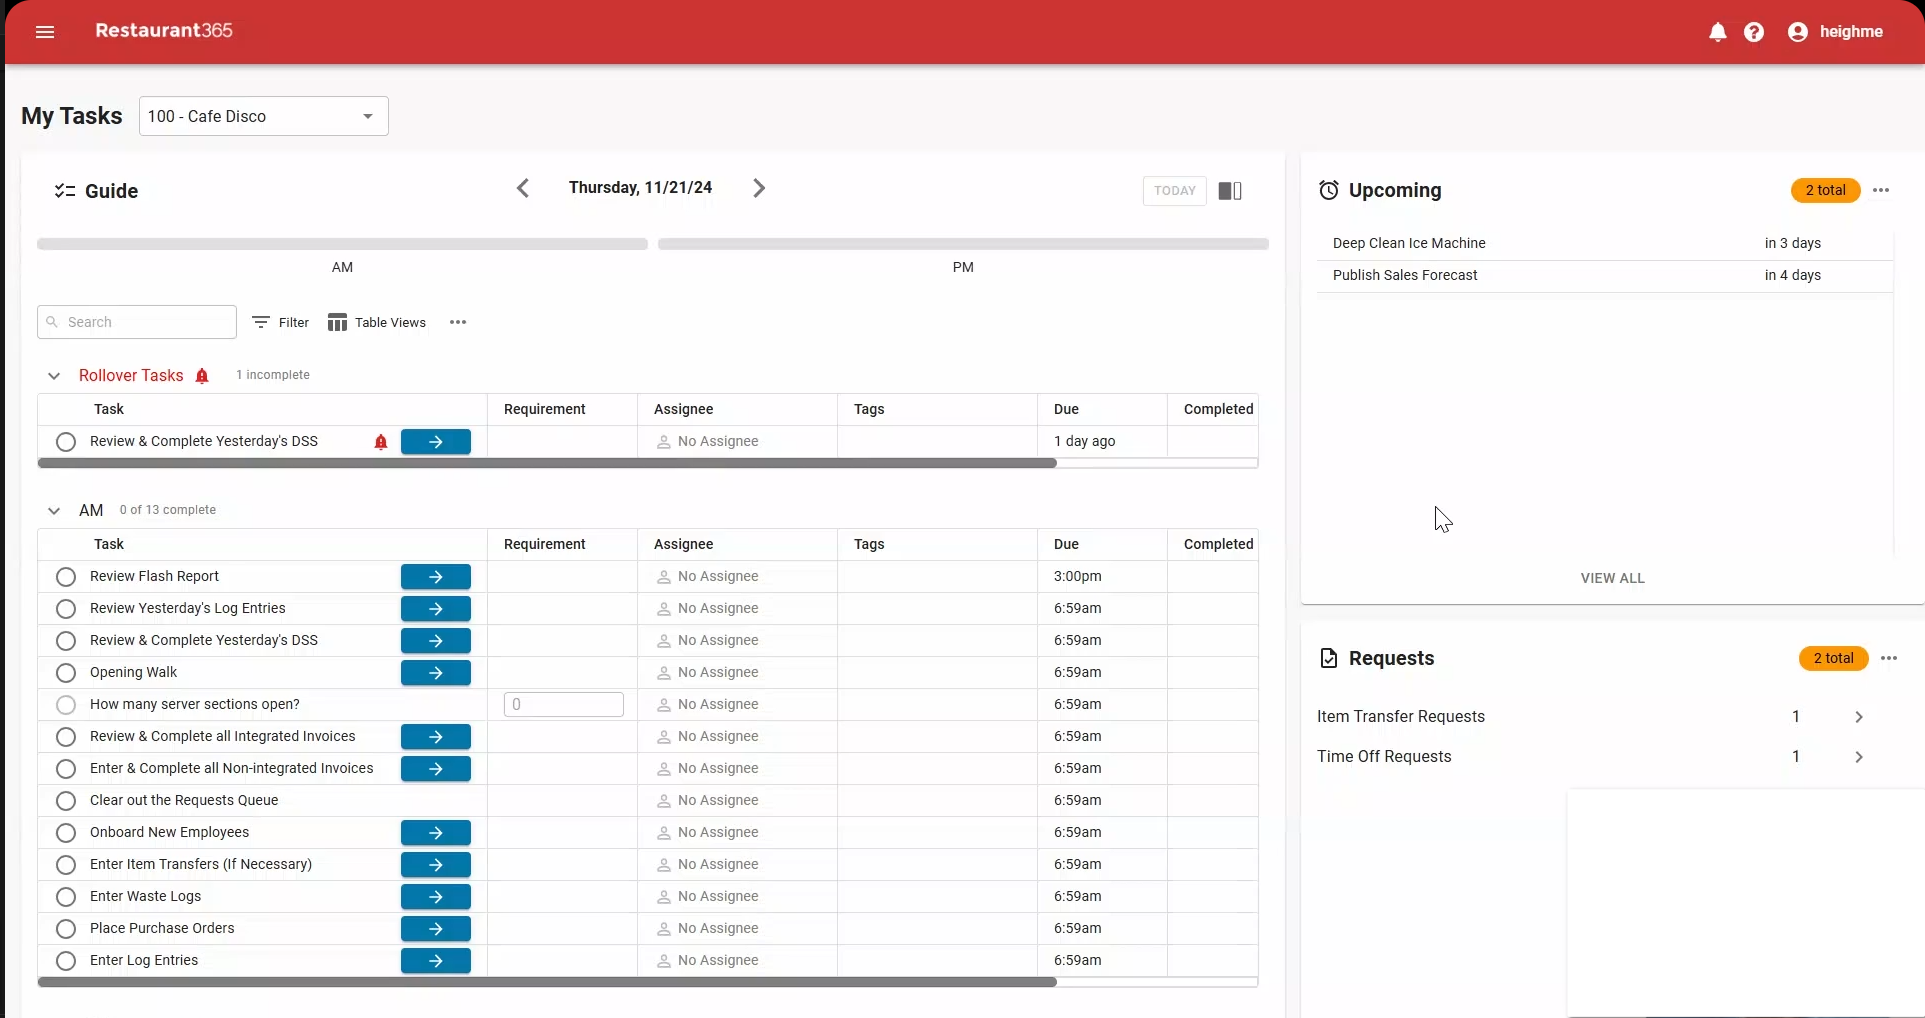
\includegraphics[width=\textwidth]{images/examples/task_management_r365.png}
        \caption{Task management (Restaurant365)}
    \end{minipage}
\end{figure}

\begin{figure}[h]
    \centering
    \begin{minipage}{0.48\textwidth}
        \centering
        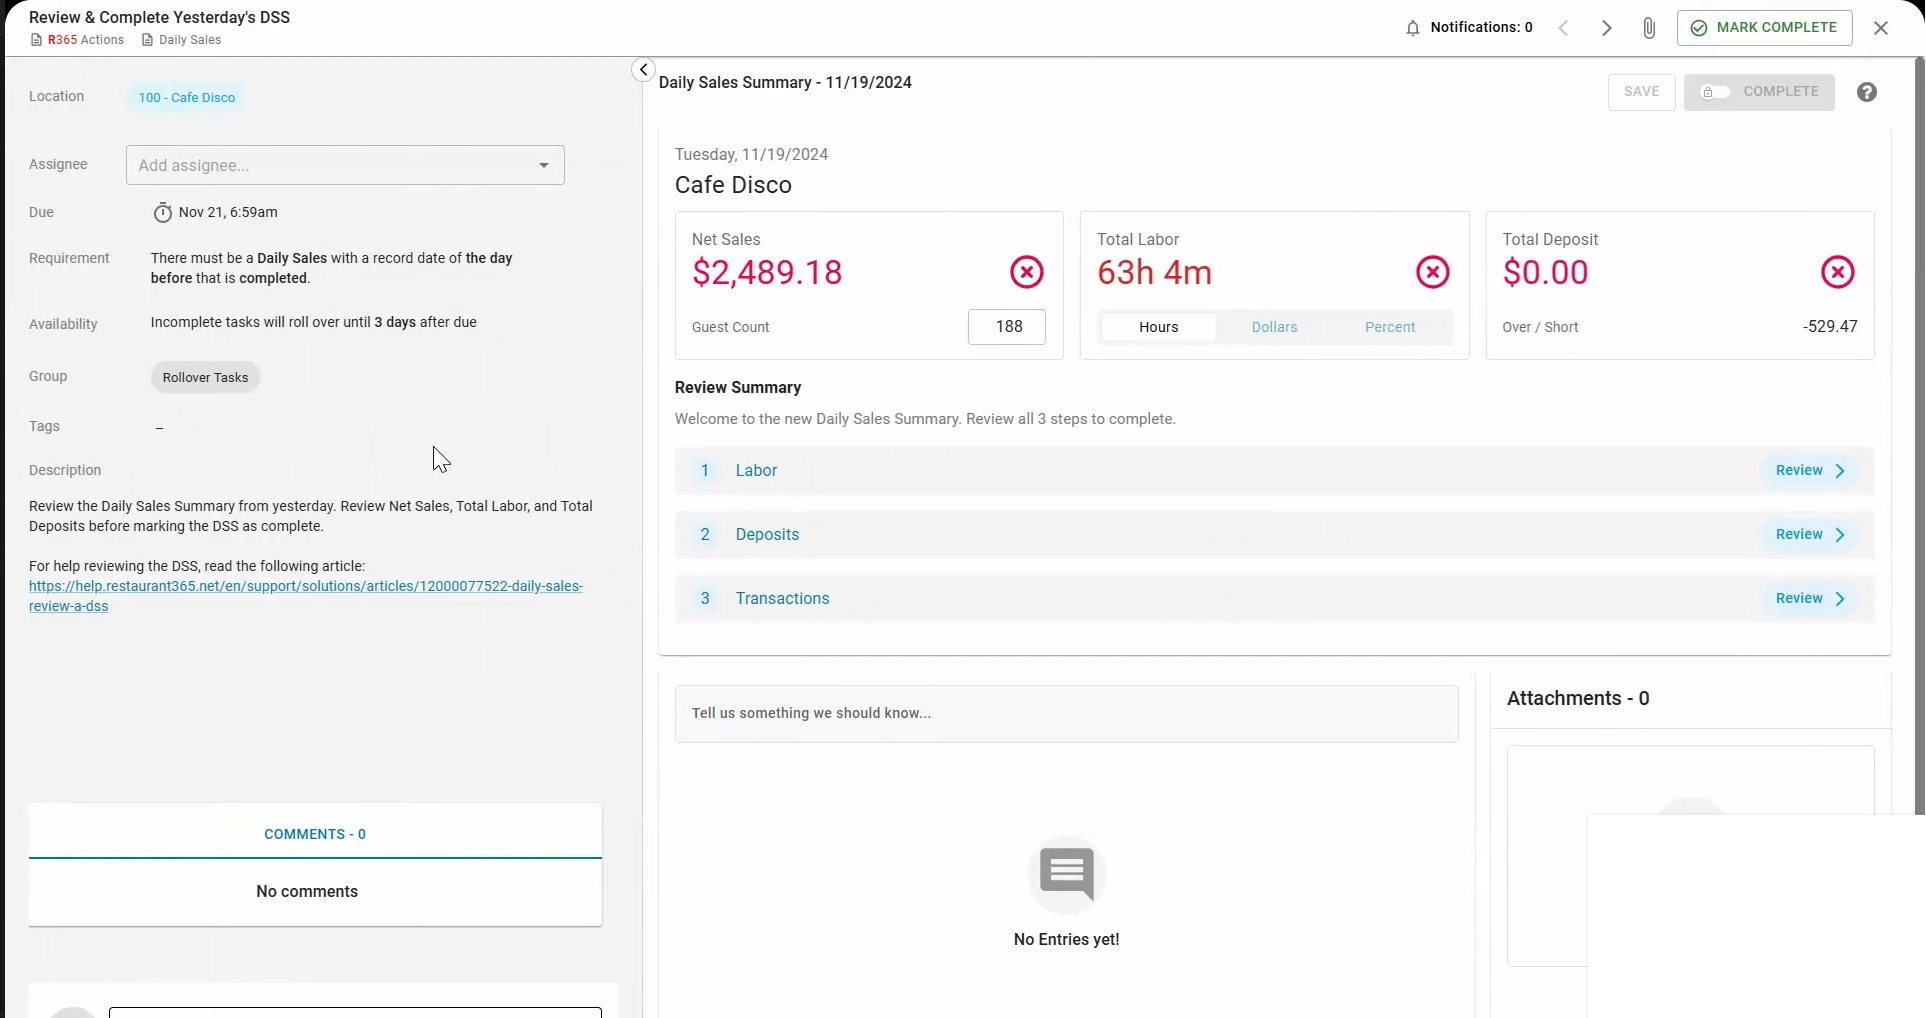
\includegraphics[width=\textwidth]{images/examples/task_review_r365.png}
        \caption{Task review interface (Restaurant365)}
    \end{minipage}
    \hfill
    \begin{minipage}{0.48\textwidth}
        \centering
        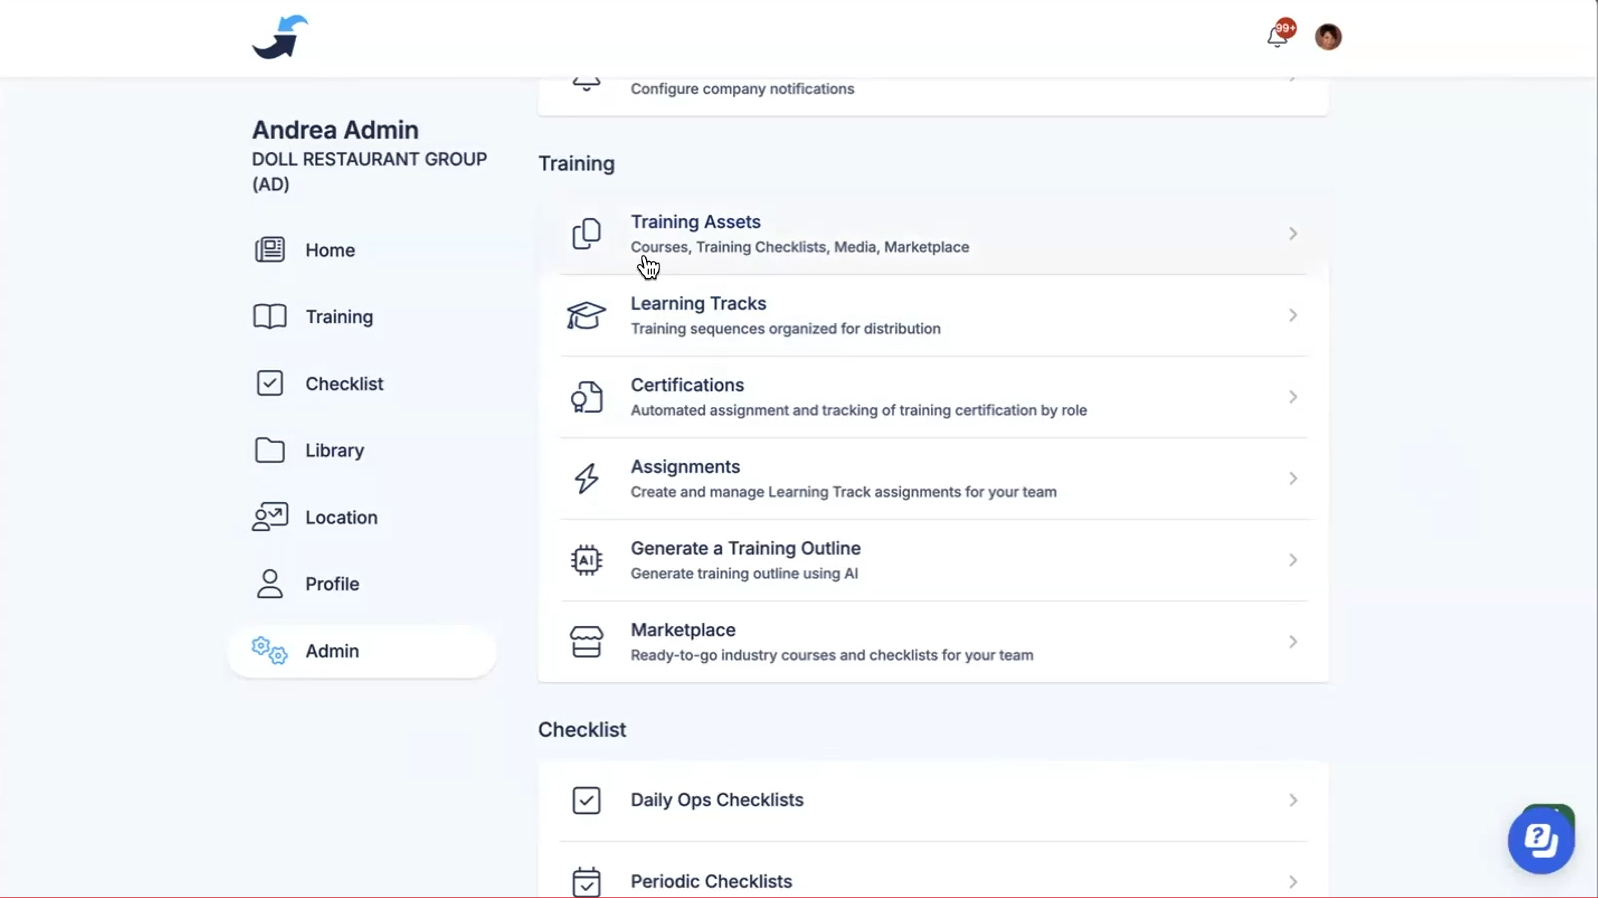
\includegraphics[width=\textwidth]{images/examples/trainings_r365.png}
        \caption{Training modules (Restaurant365)}
    \end{minipage}
\end{figure}

% sestadieni reikes ikelti.

% didinti verslinguma nera poreikis, nebus tokio mygtuko

% tarpininkas turi gauti kazkokius notifications
% poreikiai bus padavejo GUI.

% tam tikros funkcijos ateis is pasakotojo pasakojimo, atsekamumo matrica
% customer nera usability objectives, nes jis naudoja per tarpininka, sita
% reikia pamineti.

% ook for existing design examples that could inspire future design solutions
% (at least 5). - geri is kitu sistemu, screenshot, kuriai funckijai cia galetu
% tikti, kodel manom kad otks dizainas tiktu.


% paziureti kaip needs rasomi pagal standarta, skaidrese, angliskai ir
% lietuviskai kazkur parasytas paaiskinimas

% atsekamumo matrica -  viena galima vienam dalykui, kita kitam. atsekamumas
% turi parodyti kad poreikis is kazkur isplaukia, is kurio scenarijaus, is kurio
% pasakojimo, is kurio user story.

% jeigu rasome kaip sekmes kriteriju kad turi vartotojas gauti kazka per viena
% min tai reiskia kazkur parasyta kad adabar jis ta gauna ilgiau nei viena min.


% tekste paveiksliuka pacituoti, pasakyti kodel jis yra ten, koks poreikis.

% ------------------------

% primari ir secondary stakeholder kursime sasaja
% poreikis - ka veiks vartotojas ir ka gaus ekrane




% ------------------------



% ------------------------
% PACT stuff below
% ------------------------



% reikia sistemizuoti kokioje situacijoje ko reikia, labiau detaliau issiaiskinti stakeholder needs.
% reikia atlikti naudojimo konteksto analize, kaip tos funkcijos isilies i vartotojo esama gyvenima. Mes galvojame apie naudojima ir konteksta vis dar.
% Naudojimo kontekstas - kaip veiklos itakoja technologiju kaita ir technologiju kaita veiklas, po to kalbesime apie pagrindines zmoniu charakteristikas, kas, kokiose veiklose ir problemas kurias norime spresti, kokiame zingsnyje kas ten stringa, kokioje aplinkoje ten vyksta, kokios tech naudojamos ir ka galime pasiulyti.
% Naudojimo kontekstas - kombinacija vartotoju, uzduociu, resursu, tikslu. Fizines, socialines, technines, kulturines, organizicines aplinkos. Jas riekes issaiskinti ir aprasyti kaip dabar veikia tas vartotojas, ka tie pasakojimai turi atspindeti: turi buti aiskus visi aspektai, kas, kokie tisklai, aplinkos, kokiais prietaisais, programomis naudojasi ir t.t.
% PS inzinerijos standartas - naudojimo kontekstas pagrindinis informacijos reikalavimu saltinis.
% Vystimasis yra begalinis ciklas, yra zmones betkokio amziaus, kutluros, jie veikia kazkokiam kontekste (requirements), tame kontekste kyla nauji reikalavimai naujoms technologijosm, naujos technologijos sudaro galimybe keistis veiklos, vel atsiras nauji reikalavimai ir t.t. gaunasi begalinis ratas.
% naujos interaktyvios tech - prisidedame dabartines zinias, sukaupta patirti ir kuriame naujus reikalavimus. Suvokdami kazkokius nepatogumus, koks yra stovis, kokias galimybes mes galime isnaudoti su technologijomis mes pasiulome sprendimus, naujas veiklas.

% People, context, activities, technologies

% ____________________________

% People - kokiomis salygomis veikia, ju fizines galimybes, darbo vieta, veikimo
% aplinka kur bus naudojama technologija, zmoniu ugis, aukstis, antropronetiniai
% dalykai? ivestis isvestis, klaviaturos ir t.t. Nera vidutinio vartotojo,
% universali technologija reiskia kad visiem patogu naudotis, zinoma yra tam
% tikri kompromisai, reikalavimai turi tilpti i budget. Pvz.: ekrano padetis,
% ryskumas, kontrastas, color blindness, motion sensitivity, hearing etc. etc.
% Musu varottoju tarpe jeigu yra vyresni zmones tai turime i tai atsizvelgti,
% mygtukai didesni ir t.t. Kokia turi buti darbo aplinka kad zmogus nepavargtu,
% nebutu broko, darbo vieta turi buti tokia kuri leistu islaikyti darbinguma.

% psihologinis erdviu suvokimas, kai kurie pasiklysta, kai kurie gerai
% orientuojasi erdvese. kalbos skirtumai, kai kam gali buti izeidzianti kalba,
% kai kam ne...

% isiminimas, trumpalaikis isiminimas, sprendimu priemimas, komunikacija,
% paieska - mes turime sias veiklas kurioms kuriame technologijas.

% socialiniai skirtumai - itakoja motyva pirkti nauja technologija, gali
% atsirasti stiprus motyvas, pvz bendrauti nuotoliniu budu, todel zmones ismoks
% tai. skirstosi tipai, begginer, inermediate, expert zmoniu. pvz bileteliu
% popieriniu nenupirksi, tai beggineriai turi tai naudoti... vidutiniskai patyre
% kai reikia tia naudoja o taip tai nenaudoja. profesionalai - kiekviena diena
% naudoja. beggineriu ir expertu poreikia yra labai skirtingi.

% kad pradedantysis galetu naudotis technologija tai ji turi vesti uz rankos,
% pvz vedlys, jis vedamas uz rankos.

% ekspertai - jiem reikia greicio, juos vedlys erzins.

% vidutiniskai patyre - reikia prisiminti greitai.

% jie visi turi skirtingus poreikius, reikia suprasti su kuo turime reikala.


% Mental model - mintinis modelis, koki vaizda suformavo vartotojas savo
% galvoje, mes bandome tai sufprasti, tai suvokimas kas ir kaip gali naudoti
% technologijas. Mintinis modelis nepilnas, nestabilus, mes negalime visko
% prisiminti, kazkas isilaiko ilgalaikeje atmintyje, kazkas dingsta.
% Analizuojame o ka dabar naudoja vartotojai, analizuojame ju mintines zinias.
% Mintinis modelis kuriamas saveikaujant su sistemomis, su kokiomis sistemomis
% saveikauja toki ir turesime mintini modeli.

% Nustatymas vartotojo igudzius yra musu tikslas. kokio amziaus, lytis, fizines,
% issilavinimas, kulturinis, motivacines galimybes, tikslai, asmenybe.
% Projektavimo tikslai turi susieti su tais skillais. musu tikslas kad
% vartotojai pilnai isnaudotu ka suprojektavome, norime kad is begginer greitai
% pereitu i intermediate.

% Pavyzdiziui kai pirma karta paleidziame programa, gali issokti gidas, padeti
% beginneriams, o kam nereikia tai gali uzdaryti, uzdaro vidutiniskai patyre.
% Ekspertam reikia kuo greiciau dirbti, kas stabdo (rankos kelimas nuo peles iki
% klaviaturos, galime sakyti kad viska darytu ant klaviaturos).

% kiek tu sluoksniu design reikia? tai papildomos islaidos ir t.t.


% begineriam programa turi pasakyti ka ji gali daryti, pagrindiniai dalykai ka
% ji daro, begineriu nera daug bet jie yra ir pirmi naudotojai todel jiems
% reikia viska paaiskinti. po keliu kartu dauguma begineriu tampa intermediate.
% intermediate svarbu matyti, isnaudoti visas funkcijas kurias jie zino kad yra,
% gebeti viska surasti, pazengusias funkcijas. GUI visas pagrindines ir
% pazengusias funkcijas rodo ir galima greitai surasti Ekspertu nera daug,
% kazkam galbut greiciau reikia.

% kuri viekla daznesne, ta turi buti arciau ekrano.


% Universal usability - prieinamas visiems, ir neigaliems. Panaudojamumas +
% prieinamumas = universalumas. kas aktualu, kam kuriame sistema, i sita turime
% atsakyti.



% Reikia pamineti demographics, age, occupation, gender (jei reikia),
% disabilities. Motyvacija ismokti technologijas, jomis naudotis. Naudojamos
% technologijos ir prietaisai, IT lygmuo, skillai.

% ____________________________

% Veiklos - reikia ne specifines mineti, o laiko aspektu daznas ar retas,
% bendradariavimo aspektus, individualus ar organizaciniai, tos veiklos
% sudetingumas, pasekmes, ar kritines, kokio tipo turinys toje veikloje.

% Daznis jos pirma charakteristika, jos trukme antra, laiko spaudimas, ar veikia
% ramybes busenoje ar skubos. Ar tai viena atomine veikla ar zingsniai yra, ar
% testine is zingsniu tai kazkuriame zingsnyje vartotojas gali sustoti. atsako
% laikas. Bendradarbiavimas, vienas ar grupeje, kaip zino kas ka padare, kaip
% koordinuoja, komunikuoja. Sudetingumas veiklos, ar veikla apibrezta ar ne,
% reikia suteikti vartotojui galimybe narsyti ivairias veiklas, kur vartotojas
% nori narsyti, kaip vartotojas supras ar nutrauke zingsni ir t.t. tai
% sudetingumas. kaip supras kad klaida padare, ar tai aktualu. kokie duomenys
% vaiksto, kiek ivesti ten reikia, kokia ten isvestis dabar ir kas siuloma, turi
% buti realiu laiku atnaujinamas turinys, kad nebutu blogai pavaizduotas, blogai
% atnaujintas.

% Ne pacios veiklos idomios bet ju charakteristikos.

% ____________________________

% Aplinka - fizine, kur vyksta ta veikla, patalpoje, uz patalpos, jeigu fizine
% aplinka lauke, tai skirtinga temperatura, kaip vartotojas su pirstinemis ar
% per lietu gali naudotis, apsvietimas, triuksmas ir t.t.

% Socialine aplinka - individuali, o gal grupine, ar privatumas aktualus, ar
% visi vienodu teisiu, ar yra super adminas.

%  Organizacinis kontekstas - teises ir t.t.

% ____________________________

% Technologijos - ka dabar naudoja zmones, kokias technologijas, ka jie dabar naudoja, tia itakoja ju mintini modeli, kaip jie dabar iveda informacija?

% Kokias technologijas naudosime - kompiuteris, programele telefone, ar t.t.

% Turime susivokti kokiu techniniu ir sistemu reikia. Kas yra geras turinys ir kokios charakteristikos galetu tobulinti tai, balsu ivedimas, AI ar whatever.

% kokia informacija ir funkcijos reikalingos sistemai, kas tures buti zinoma norinciam naudotis sitema.


% Interaktyvus produktas turi atitikti tai ko nori zmones, jis negali sugriauti kontekto, jis turi tai pagerinti.

% musu uzdavinys visus siuos dalykus issiaiskinti, parasyti kiekvienai pirminei ir antrinei vartotoju grupei aprasyti siuos dalykus ir po to dar kitai savaitei galime pradeti rasyti poreikius kas isto isplaukia ir kokiu funckiju riekia

% \sectionnonum{Results and conclusions}
% For details of what needs to be written in this section, please refer to the methodology requirements of the respective programme.


% ------------------------
% User Studies
% ------------------------

% Suvokimo procesas - nelabai gali issivaizduoti, projekte vyksta kuryba.
% Jeigu viskas patogu tai niekas nepastebi, jeigu kazkas nepatogu tai visi pastebi..

% Yra PACT sistema kuri apibendrina viska. Patys bendriausi reikalavimai yra
% vartotoju poreikiai, tai nevisai kaip reikalavimai. Poreikiai - ka vartotojas
% nuveiks, ka matys sistemoje.

% Vartotojau nori kad processas butu sklandus, intuityvus <- negeras aprasymas,
% ar cia bus mygtukas ar kazkas ekrane, cia yra labiau verslo lukesciai.



% Scenarijai turetu pateikti zingsnius kaip vartotojai dabar veikia, 
% what
% how
% any problems /\<- visa sita jau padarem

% ------------------------
% Koki tyrima darom
% yra kokybiniai ir kiekybiniai tyrimai
% kiekybiniai - apklausos, anketos, statistika, daug zmoniu, galime apibendrinti visai populiacijai, bet gauname mazai izvalgu
% kokybiniai - interviu, stebejimas, mazai zmoniu, gauname daug izvalgu, bet galime atsidurti klaidingoje situacijoje, negalime apibendrinti visai populiacijai


% kiekybiniams reikia didelio biudzeto.

% kiekybiniame tyrime suzinome nuostatas, problemas su laiku pradeda kartotis info.


% human centered design - suzinome prie ko zmones priprate ir atitinkamai
% kuriame technologijas. kokios veiklos daznos, retos, danzesnes veiklos
% pradiniame ekrane, retesnes kitame, etc.


% PERSONAS - isgrynina visas iskalbas kalbant su tam tikra vartotoju grupe.
% persona gaunama pakalbant bent su keliais atstovais is tos vartotoju grupes.
% persona yra konkretus atstovas skirtingu vartotoju grupiu.
% tikslai, prasmingos veiklos isskiriamos.


% zmones kurie daug zino ir kurie nenaudoja mainstream technologijas yra geras
% info saltinis. nereikia kalbeti su mainstream, uzkart galime suzinoti kas
% blogai su tuo mainstream. Gausime gera izvalga, kokie trukumai su ta
% mainstream technologija.



% 1 setting goals - atlikti PACT analize 

% 2 identifikuoti dalyvius, nuspresti is
% ko rinkti info (suinteresuotu analize jau atlikome), probability sampling
% (paimame atsitiktiniu budu zmones) arba non probability sampling (krastutiniu 
% grupiu). Saturation sampling - su visais kalbame kol nebelieka naujos info.

% 3 Relationship with participants - susitarti su vadovybe kad galime kalbinti
% zmones, virsininkas turi pristatyti kad bus toks tyrimas, etc. etc. Informed
% consent - pasiraso kad sutinka dalyvauti.

% 4 Triangulation - vienas info saltinis mazai, turi buti bent keli scenarijai,
% kad zinotume skirtingus poziurius, juos derintume.

% 5 Pilot studies - pabandome su vienu ar keliais zmonemis, kad pamatytume ar
% viskas ok, ar klausimai aiskus, ar suprantami.


% Interviews

% Pirma buna nestrukturizuoti, kuo toliau tuo labiau strukturuoti, tikslinames
% funkcionalumus, pozymius.

% semi strukturuoti - yra pagrindiniai klausimai, bet galima klausti ir papildomai

% group inteviesws - diskusijos, su keliais kalbam.

% vengti ilgu sakiniu, ar, ir, zargonu, vengti stumti i viena ar kita puse.

% fokuso grupe - atstovai is skirtingu grupiu, kai isriskeja skirtingi
% poziuriai. reikia kompromisiniu sprendimu.



\printbibliography[title = {References and sources}]

\end{document}

